% !TEX root = ./main.tex
% !TEX encoding = UTF-8 Unicode
% !TEX program = pdflatex
% !TeX spellcheck = it_IT

\graphicspath{{Immagini/},{Immagini/ffda/}}

\chapter{Field Failure Data Analysis}
La \textbf{FFDA} è effettuata sui dati relativi ad un sistema in
esercizio(\textit{on Field}), al fine di scoprire i possibili fallimenti.\\
L'approccio utilizzato nella FFDA prevede di monitorare il sistema in esecuzione,
misurando parametri di dependability e prelevando tutte le possibili informazioni
sul fallimenti rilevati.\\
Un fallimento è una deviazione del comportamento del sistema dal suo corretto e
specifico funzionamento.\\
La metodologia FFDA è basata su tre fasi fondamentali:
\begin{itemize}
  \item \textbf{Data Logging \& Collection} - consiste nella definizione di cosa
  collezionare e come farlo;
  \item \textbf{Data Filtering \& Manipulation} - consiste nella manipolazione ù
  dei dati collezionati, utilizzando \textit{filtering} e \textit{coalescence};
  \item \textbf{Data Logging \& Collection} - consiste nell'esecuzione di un'analisi
  statistica su dati precedentemente manipolati, per calcolarne misure quantitative
  e identificarne possibili trends.\\
\end{itemize}

\section{Traccia}
Dati i due file di log \textit{MercuryErrorLog} e \textit{BGLErrorLog},
preventivamente filtrati per ottenere solo eventi di fallimento, si vuole:
\begin{itemize}
  \item determinare la finestra di coalescenza;
  \item raggruppare tutte le entry appartenenti alle stesse finestre di
  coalescenza(tuple);
  \item ricavare la \textit{CDF} del \textbf{TTF}(Time-To-Failure) e della
  \textbf{Reliability Empirica};
  \item fitting della CDF della reliability empirica provando tutti i modelli
  studiati (\textit{Esponenziale}, \textit{Weibull} ed \textit{Iperesponenziale});
  \item utilizzare il test di \textit{Kolmogorov-Smirnov} per controllare che il
  modello ipotizzato fitti adeguatamente i dati.\\
\end{itemize}

\clearpage

\section{Mercury}
Il sistema Mercury consiste di nodi IBM.\\
Il cluster ha un'architettura a 3 livelli(nodi \textit{login}, \textit{computation}
e \textit{storage}) ed un solo nodo di management
(\textit{tg-master}).\\
Il log è formato dai seguenti campi:
\begin{itemize}
  \item \textbf{Timestamp};
  \item \textbf{Nodo Origine};
  \item \textbf{Categoria Errore}:
  \begin{itemize}
    \item DEV, PRO, MEM, NET, IO, OTH;
  \end{itemize}
  \item \textbf{Messaggio}.
\end{itemize}

\subsection{Finestra di Coalescenza - CWIN}
La finestra di coalescenza, definita in secondi, definisce un intervallo temporale
in cui cadono tutti gli eventi che vi appartengono.\\
Lo script \textbf{tupleCount\_func\_CWINpy.sh}(riportato in figura \ref{coalescence_window_mercury}), con input i file \textit{MercuryErrorLog.txt}
e \textit{tentative-CWIN.txt}, è stato utilizzato per calcolare il numero di tuple al
variare della dimensione della finestra di coalescenza.\\

\begin{figure}[!htbp]
  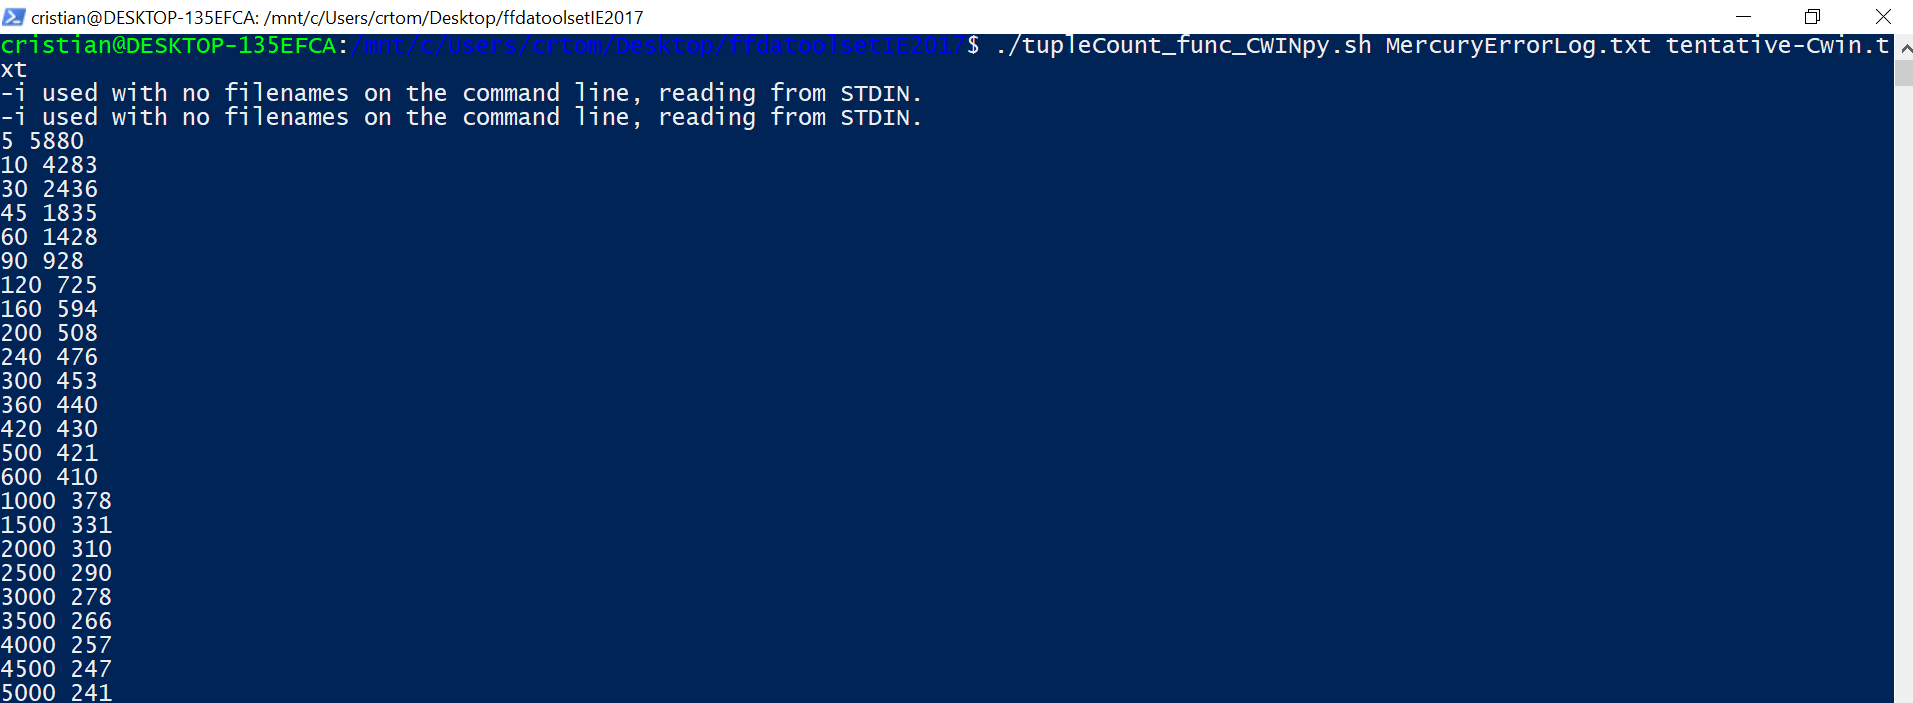
\includegraphics[width=1\linewidth,keepaspectratio]{coalescence_window_mercury}
  \caption{Script conteggio tuple al variare della finestra di coalescenza}
  \label{coalescence_window_mercury}
\end{figure}

\clearpage

L'output di tale script, plottato in matlab e presente in figura \ref{plot_coalescence_window_mercury},
è infine utilizzato per determinare un singolo valore di CWIN, ottenuto
considerando il punto successivo al ginocchio(knee) della curva.\\
Il valore di CWIN scelto è 300.\\
\begin{figure}[!htbp]
  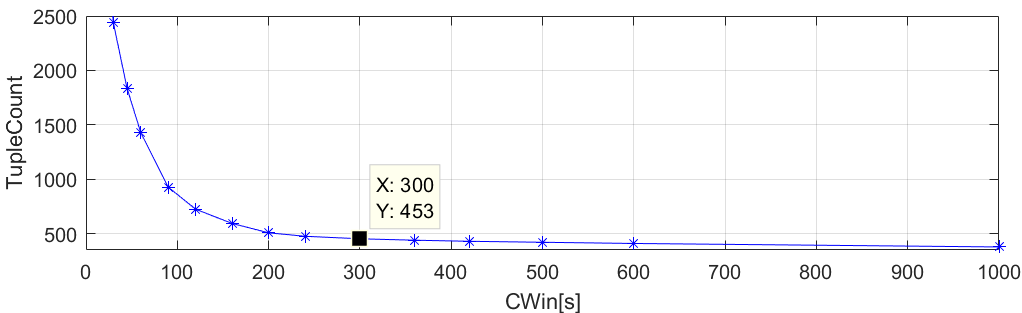
\includegraphics[width=1\linewidth,keepaspectratio]{plot_coalescence_window_mercury}
  \caption{Plot finestre di coalescenza}
  \label{plot_coalescence_window_mercury}
\end{figure}

Lo script bash \textbf{tupling\_with\_CWIN.sh} suddivide le righe del file di log,
in funzione del valore della finestra di coalescenza, raccogliendo, per ogni tupla,
le seguenti informazioni:

\begin{itemize}
  \item \textbf{Starting Points}: il timestamp della prima riga di ogni tupla generata;
  \item \textbf{Interarrivals}: il tempo che intercorre tra l'ultima riga e la
  prima riga di due tuple consecutive;
  \item \textbf{Lenghts}: il numero di righe presenti in ogni tupla.
\end{itemize}

Analizzando il file \textbf{interarrivals.txt} in matlab tramite lo script \textbf{ttf\_ref}
si ottiene la CDF empirica della TTF(Time To Failure) e dualmente la Reliability (1-TTF).\\
In figura è riportato il grafico delle due CDF.

\clearpage

\begin{figure}[!htbp]
  \centering
  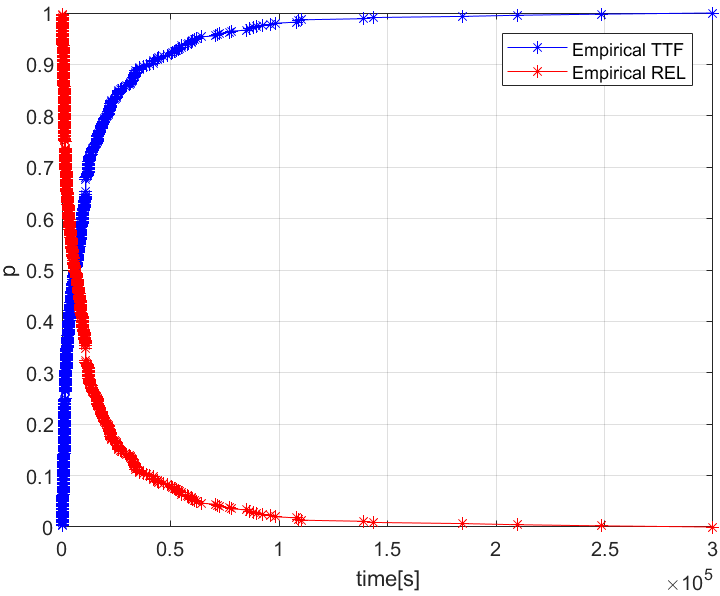
\includegraphics[width=1\linewidth,keepaspectratio]{ttf_rel_mercury}
  \caption{Plot TTF e Reliability}
  \label{ttf_rel_mercury}
\end{figure}

\subsection{Curve Fitting}

Dopo aver ottenuto la CDF della reliability è possibile procedere con il fitting.\\
Utilizzando il tool di matlab \textbf{Curve Fitting} è stato possibile
analizzare i seguenti modelli:

\clearpage

\begin{itemize}
  \item \textbf{Esponenziale}:
  $$ y = e^{- \lambda  x} $$
  Il valore $\lambda$ è stato inizializzato a $1/MTTF$.\\
  Il modello risultante in matlab è riportato nella figura \ref{Exponential_mercury}.\\

  \begin{figure}[!htbp]
    \centering
    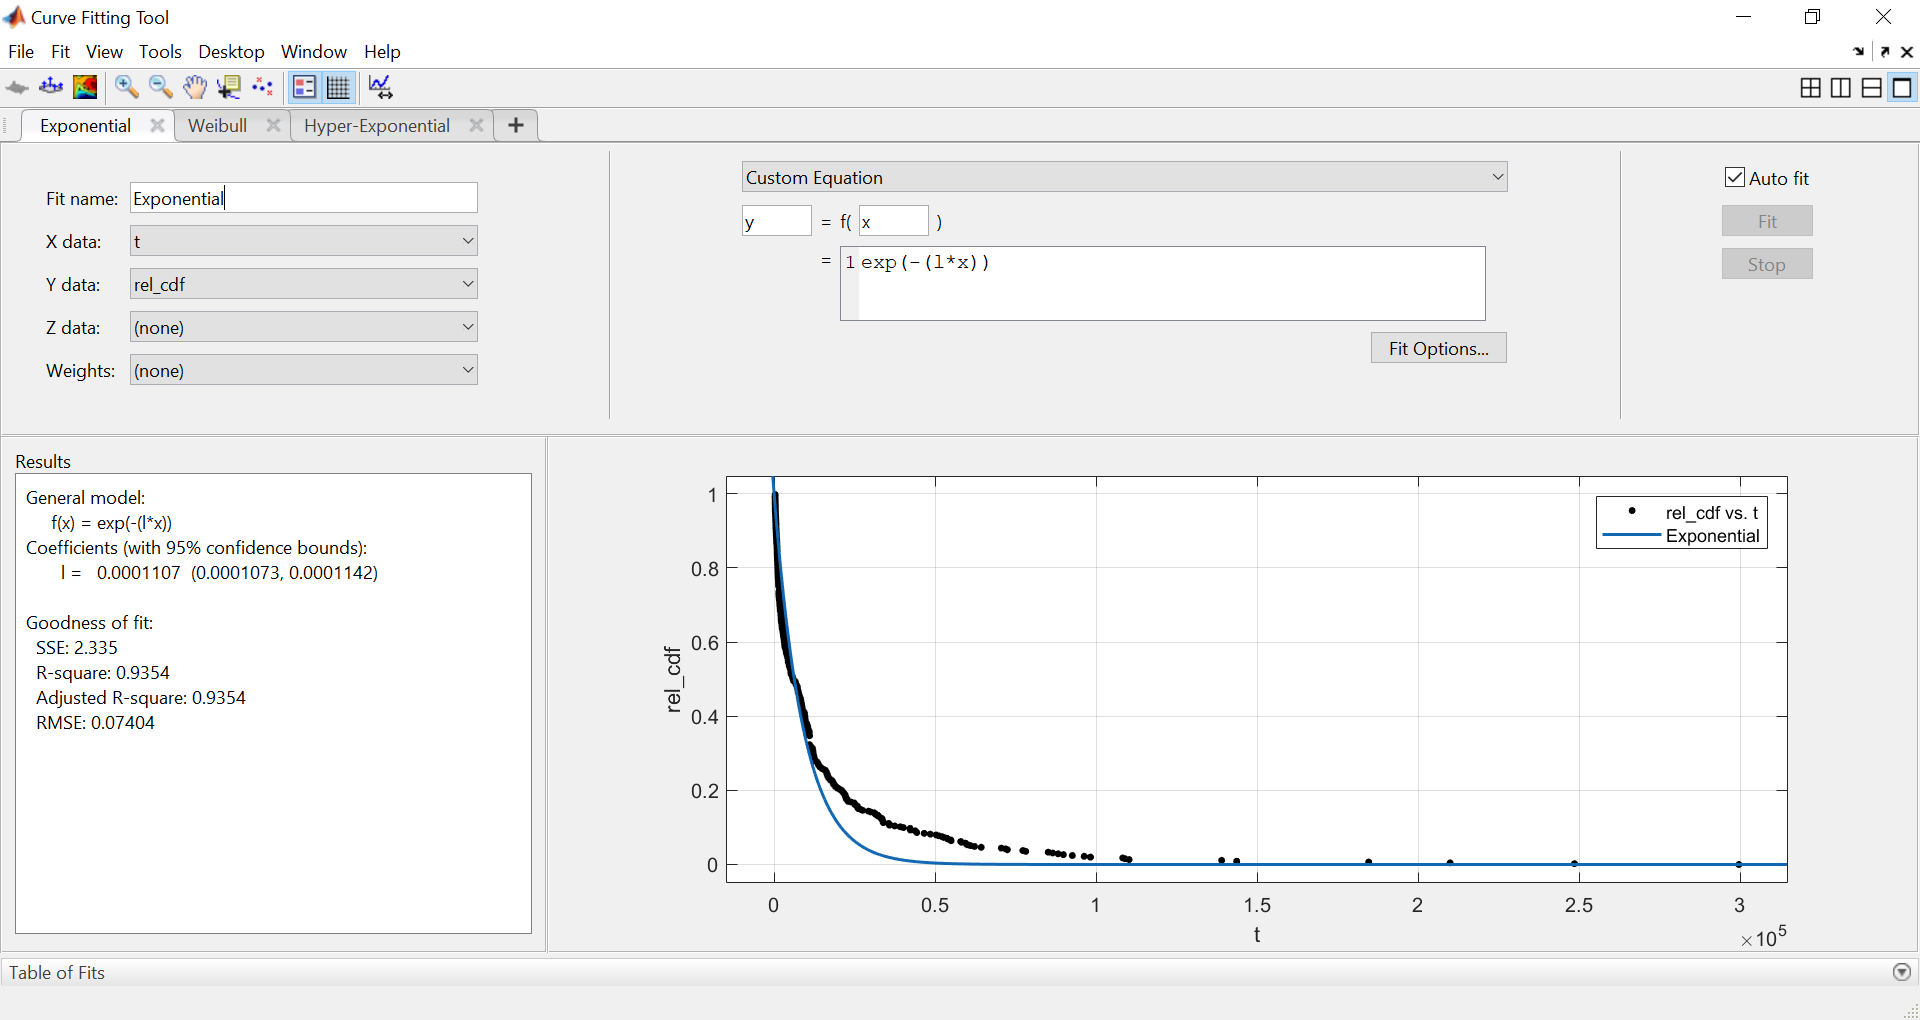
\includegraphics[width=.9\linewidth,keepaspectratio]{Exponential_mercury}
    \caption{Curve Fitting modello Esponenziale}
    \label{Exponential_mercury}
  \end{figure}

  Per valutare la bontà del fitting è stato utilizzato il \textbf{Kolmogorov-Smirnov Test}.\\

  \begin{figure}[!htbp]
    \centering
    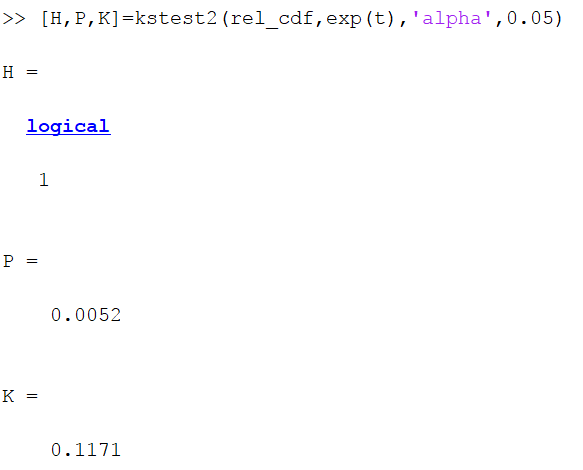
\includegraphics[width=0.5\linewidth,keepaspectratio]{ks_exp_mercury}
    \caption{Kolmogorov-Smirnov Test esponenziale}
    \label{ks_exp_mercury}
  \end{figure}

  L'ipotesi nulla è rigettata al 99,48\%, con confidenza del 95\%.

  \clearpage

  \item \textbf{Weibull}:
  $$ y = e^{- (\lambda x)^\alpha} $$
  Il modello risultante in matlab è riportato nella figura \ref{Weibull_mercury}.\\
  \begin{figure}[!htbp]
    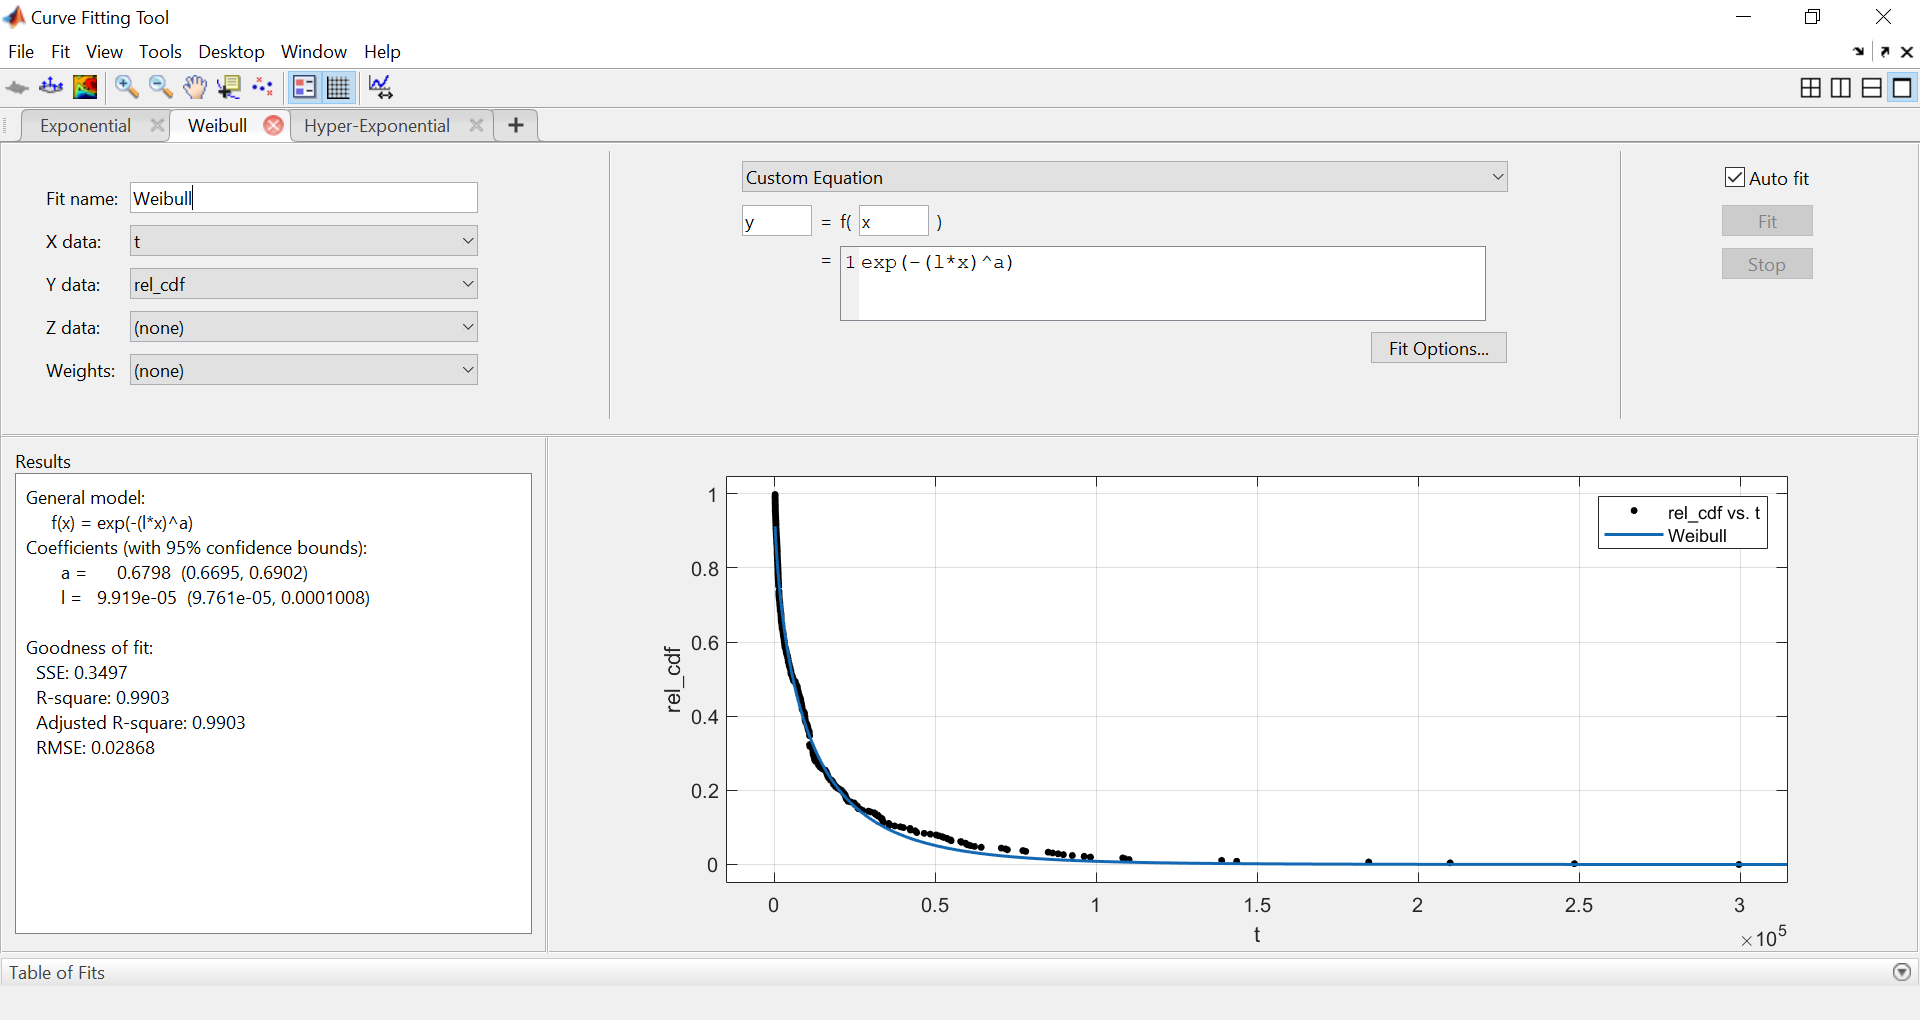
\includegraphics[width=0.9\linewidth,keepaspectratio]{Weibull_mercury}
    \caption{Curve Fitting modello Weibull}
    \label{Weibull_mercury}
  \end{figure}

  Per valutare la bontà del fitting è stato utilizzato il \textbf{Kolmogorov-Smirnov Test}.\\

  \begin{figure}[!htbp]
    \centering
    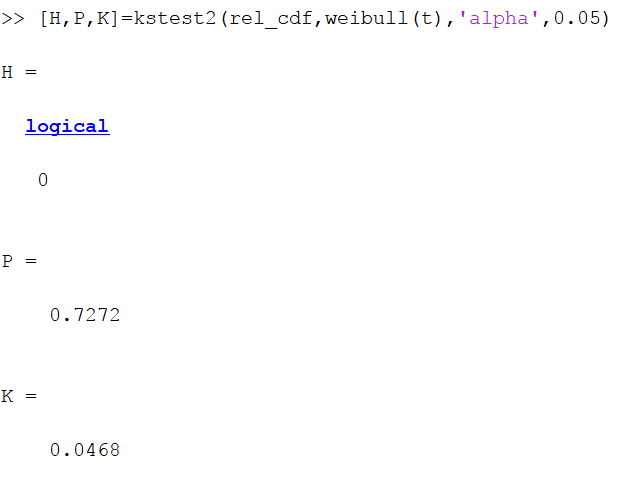
\includegraphics[width=0.4\linewidth,keepaspectratio]{ks_weibull_mercury}
    \caption{Kolmogorov-Smirnov Test Weibull}
    \label{ks_weibull_mercury}
  \end{figure}

  L'ipotesi nulla è valida al 72,72\%, con confidenza del 95\%.\\
  Quindi osservando il valore di R-quadro, è possibile concludere che il
  modello ipotizzato fitta bene la CDF empirica.\\

  \clearpage

  \item \textbf{Iperesponenziale}:
  $$ y = a e^{- \lambda_1  x} +  b  e^{- \lambda_2  x} $$
  Il modello risultante in matlab è riportato nella figura \ref{HyperExponential_mercury}.\\

  \begin{figure}[!htbp]
    \centering
    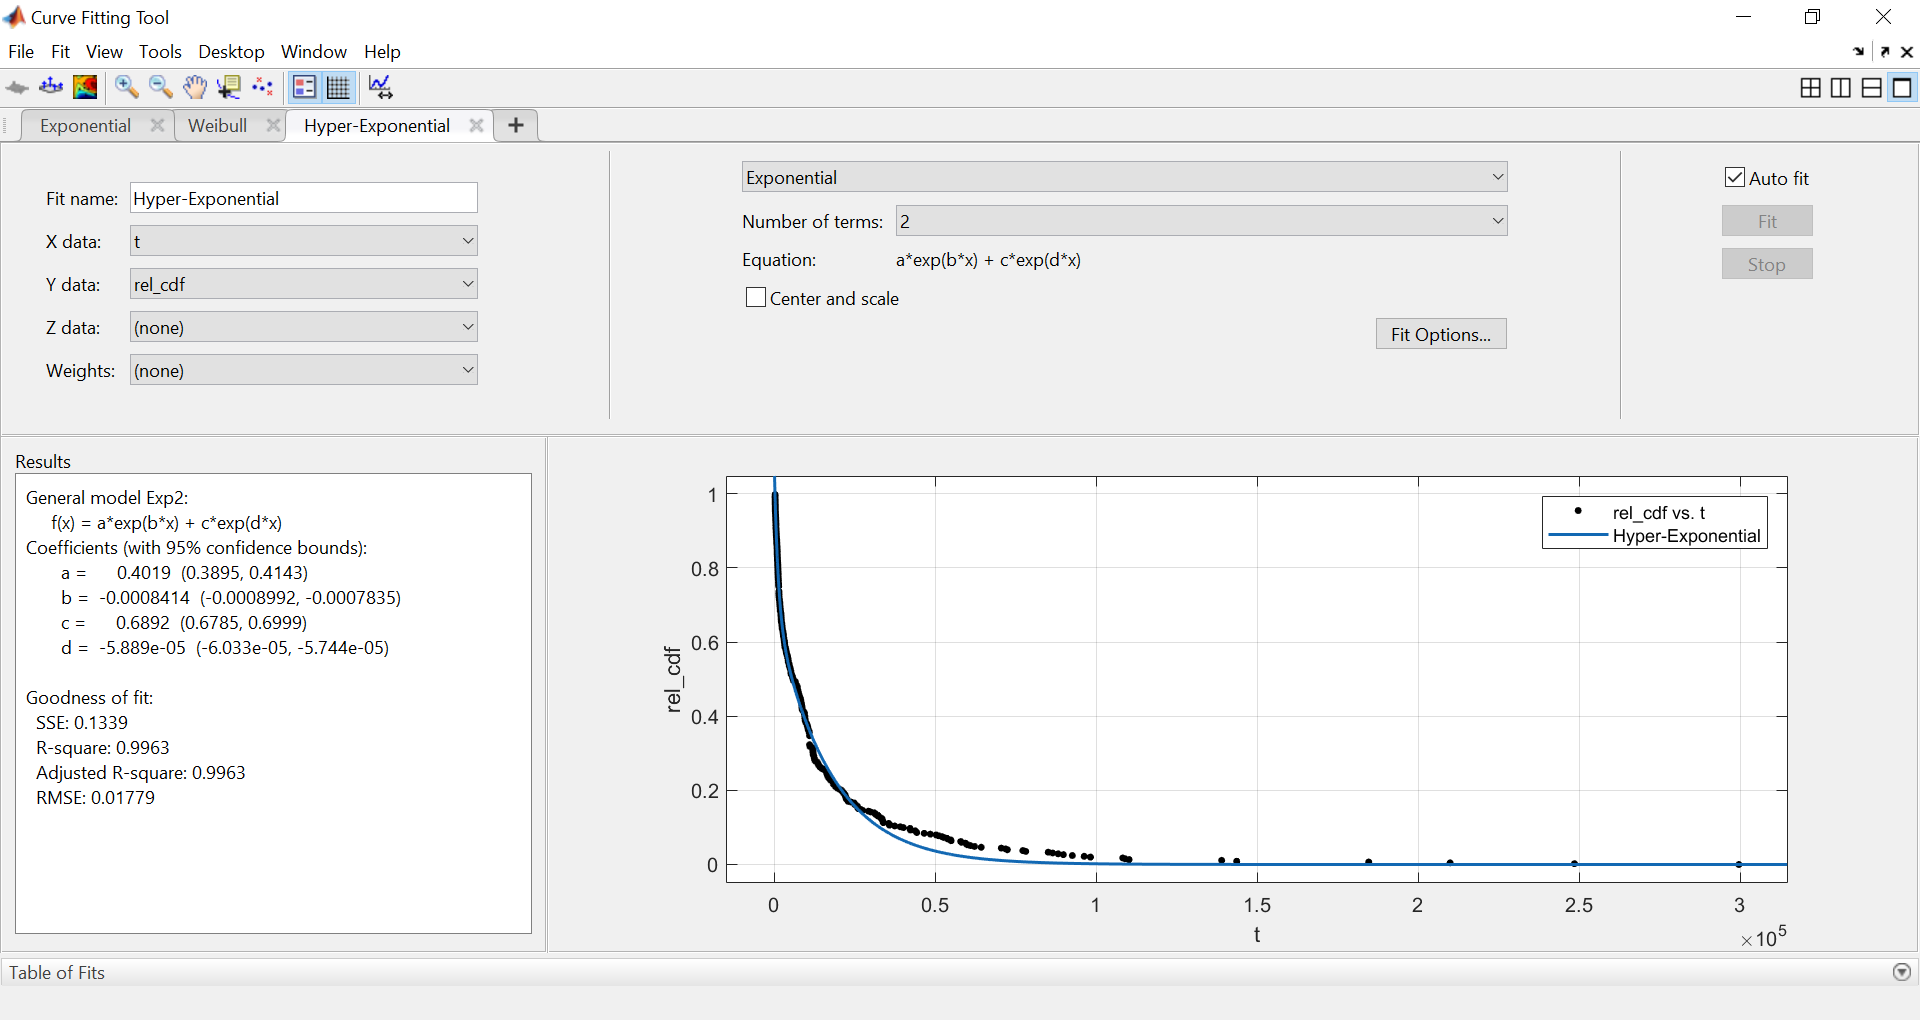
\includegraphics[width=0.9\linewidth,keepaspectratio]{HyperExponential_mercury}
    \caption{Curve Fitting modello iperesponenziale}
    \label{HyperExponential_mercury}
  \end{figure}

  Per valutare la bontà del fitting è stato utilizzato il \textbf{Kolmogorov-Smirnov Test}.\\

  \begin{figure}[!htbp]
    \centering
    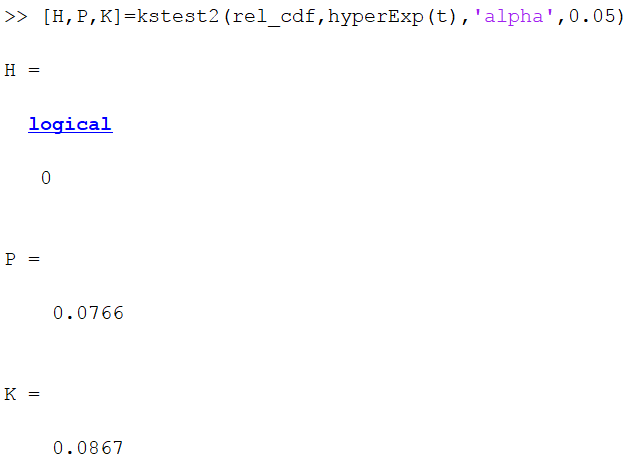
\includegraphics[width=0.5\linewidth,keepaspectratio]{ks_hyperexp_mercury}
    \caption{Kolmogorov-Smirnov Test Weibull}
    \label{ks_hyperexp_mercury}
  \end{figure}

  L'ipotesi non è rigettata al 7,66\%, con confidenza del 95\%.\\

  \clearpage
\end{itemize}

Confrontando gli R-quadro di tutti i modelli utilizzati, il migliore risulta
essere l'\textbf{Iperesponenziale}.\\
Ciò nonostante il \textbf{Kolmogorov-Smirnov Test}, nel caso del modello
iperesponenziale, non rigetta l'ipotesi nulla $H_0$ solo al 7,66\%, mentre
per il modello \textbf{Weibull}, avviene circa al 72\% .\\
Anche visivamente, il modello Weibull risulta essere quello che fitta meglio i
dati.\\

\clearpage

\subsection{Analisi del Log}
Nella figura \ref{first_5_node} è riportata l'esecuzione dello script
\textit{logStatistics.sh}, che fornisce informazioni sul numero di fallimenti
per categoria e per nodo.\\
Da quest'analisi risulta esserci un collo di bottiglia per le categorie:
\textit{DEV (57248 fallimenti)} ed uno per i nodi: \textit{tg-c401 (62340 fallimenti)}.\\

\begin{figure}[!htbp]
  \centering
  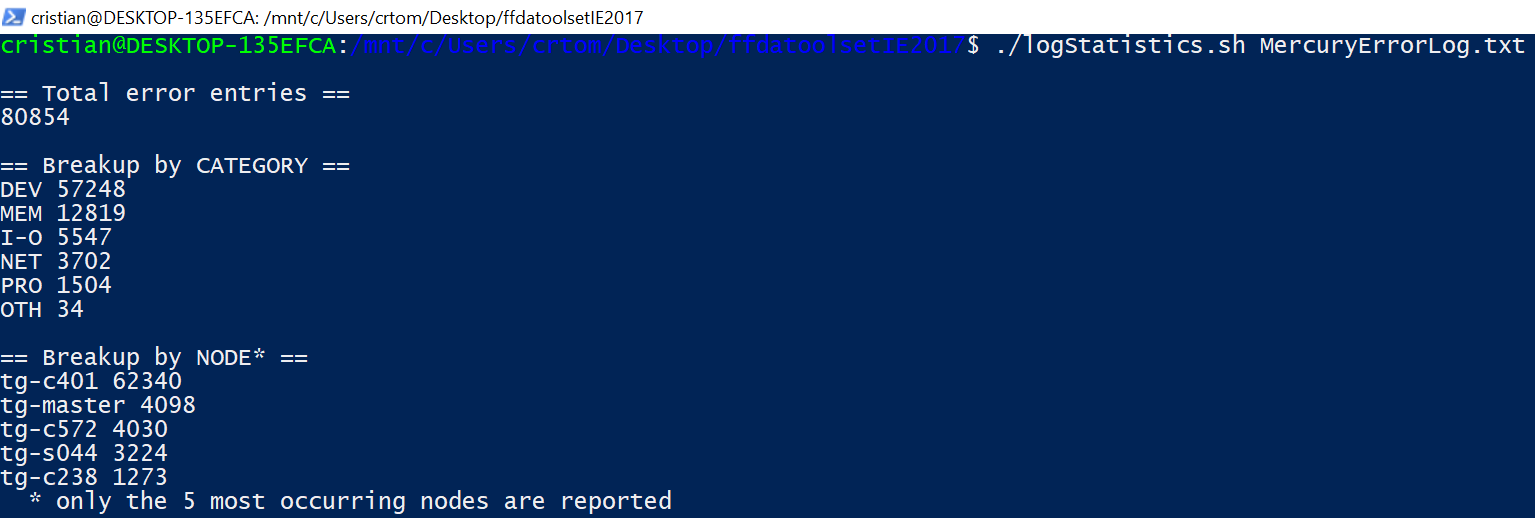
\includegraphics[width=\linewidth,keepaspectratio]{first_5_node}
  \caption{Esecuzione script logStatistics.txt}
  \label{first_5_node}
\end{figure}

In tabella \ref{nodi_dev} i fallimenti sono distribuiti sulle righe per nodo
(solo i 5 nodi più influenti) e sulle colonne per categoria.\\

\begin{figure}[!htbp]
  \centering
  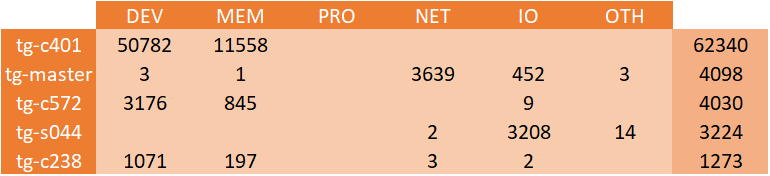
\includegraphics[width=\linewidth,keepaspectratio]{nodi_dev}
  \caption{Numero fallimenti per categorie e nodi}
  \label{nodi_dev}
\end{figure}

Dalla tabella \ref{nodi_dev} è possibile notare che:
\begin{itemize}
  \item nessuno dei 5 nodi riportati ha occorrenze per la
  categoria di errore \textit{PRO};
  \item il nodo tg-c401 presenta solo fallimenti di categoria \textit{DEV} e
  \textit{MEM};
  \item il nodo tg-master presenta, principalmente, fallimenti di categoria
  \textit{NET} e \textit{IO};
\end{itemize}

\clearpage

\subsection{Domanda 1}
\textit{La finestra di coalescenza CWIN è la stessa per tutti i nodi considerati?}

\subsubsection*{Soluzione}
Per poter rispondere alla domanda è necessario calcolare la finestra di coalescenza
per ogni log filtrato per nodo.\\
I risultati ottenuti sono riportati in figura \ref{cwin_5_nodi}.\\

\begin{minipage}{\linewidth}
  \centering
  \begin{minipage}{0.49\linewidth}
    \begin{figure}[H]
      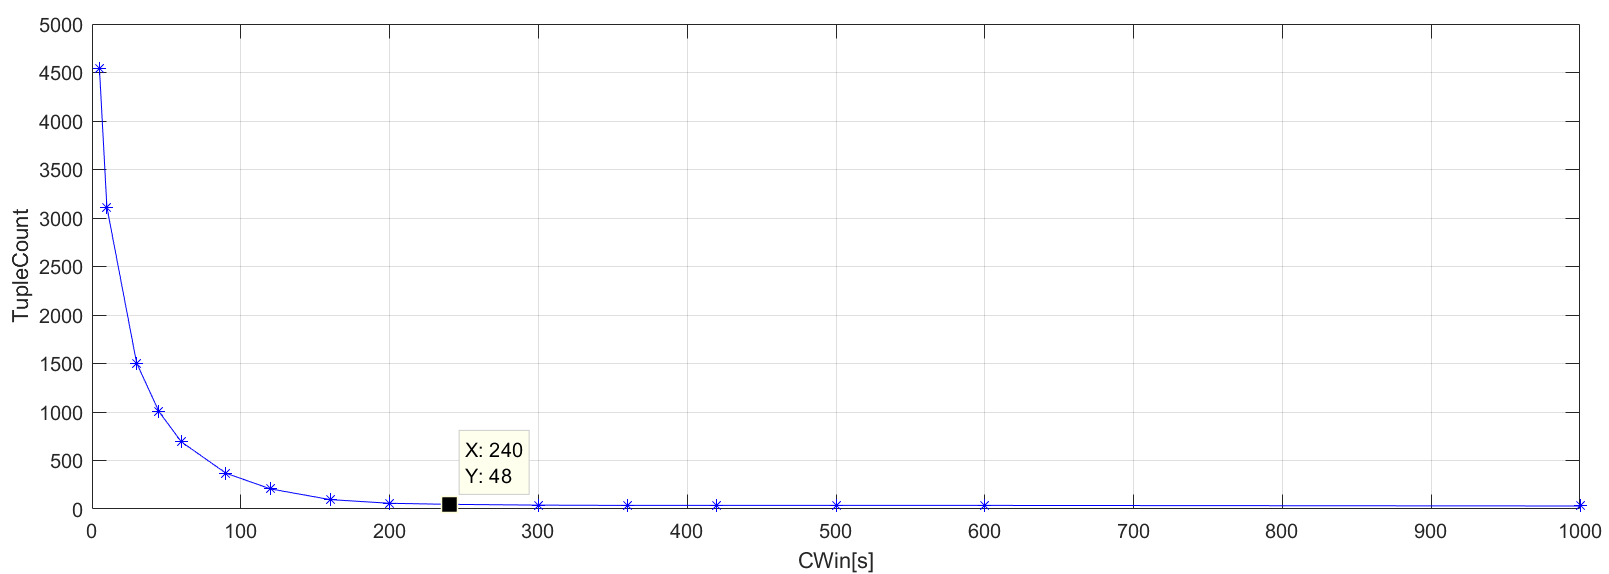
\includegraphics[width=\linewidth]{plot_tg_c401_cwin}
      \caption*{tg c401}
    \end{figure}
  \end{minipage}
  \begin{minipage}{0.49\linewidth}
    \begin{figure}[H]
      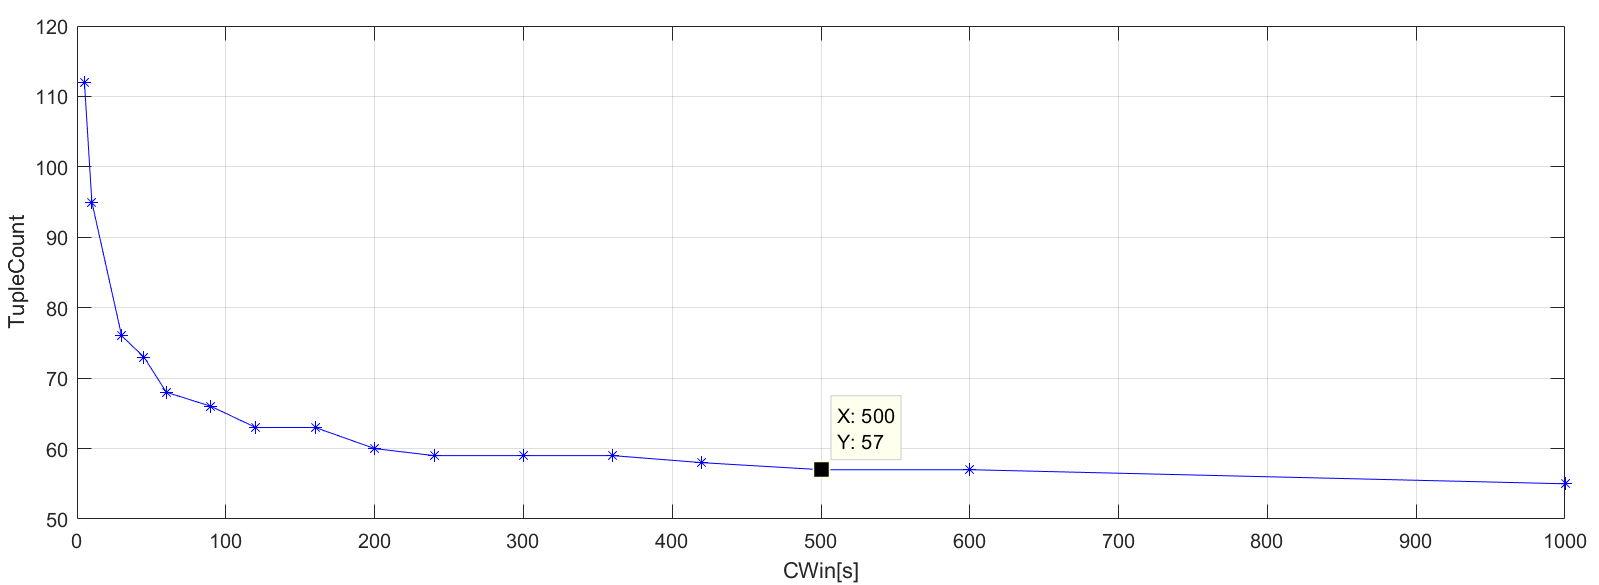
\includegraphics[width=\linewidth]{plot_tg_master_cwin}
      \caption*{master}
    \end{figure}
  \end{minipage}
  \begin{minipage}{0.49\linewidth}
    \begin{figure}[H]
      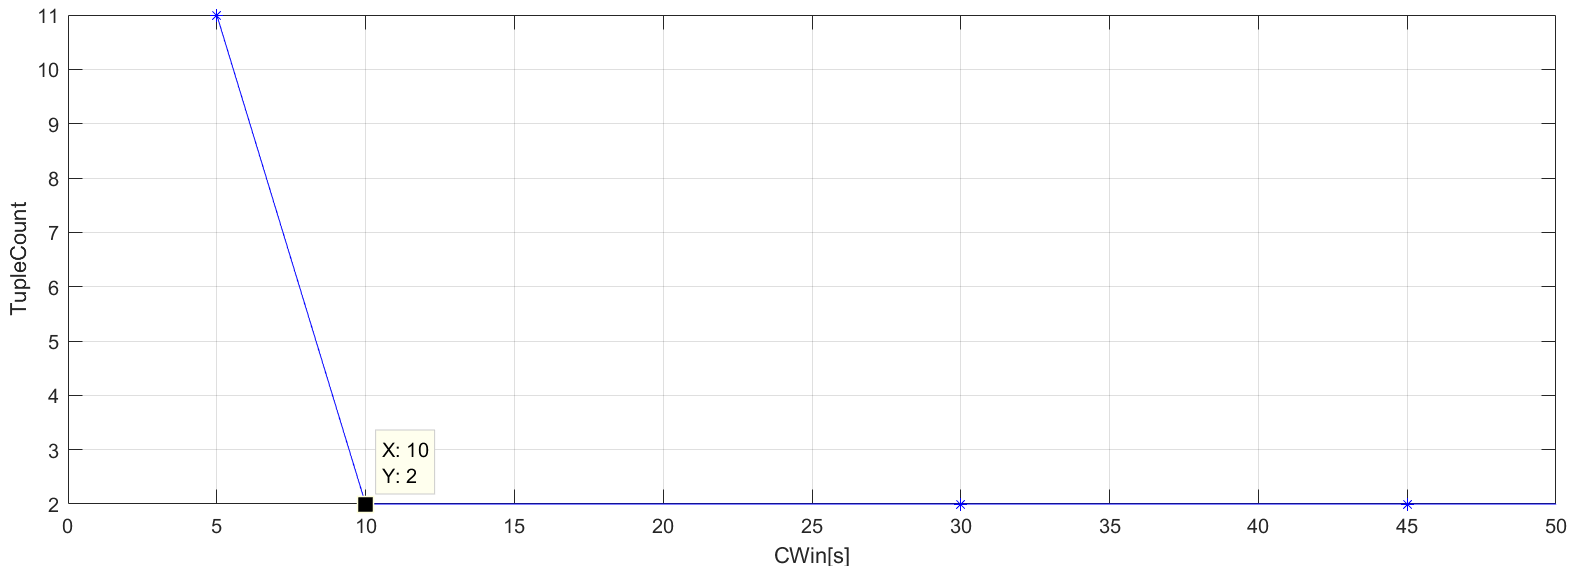
\includegraphics[width=\linewidth]{plot_tg_c572_cwin}
      \caption*{tg c572}
    \end{figure}
  \end{minipage}
  \begin{minipage}{0.49\linewidth}
    \begin{figure}[H]
      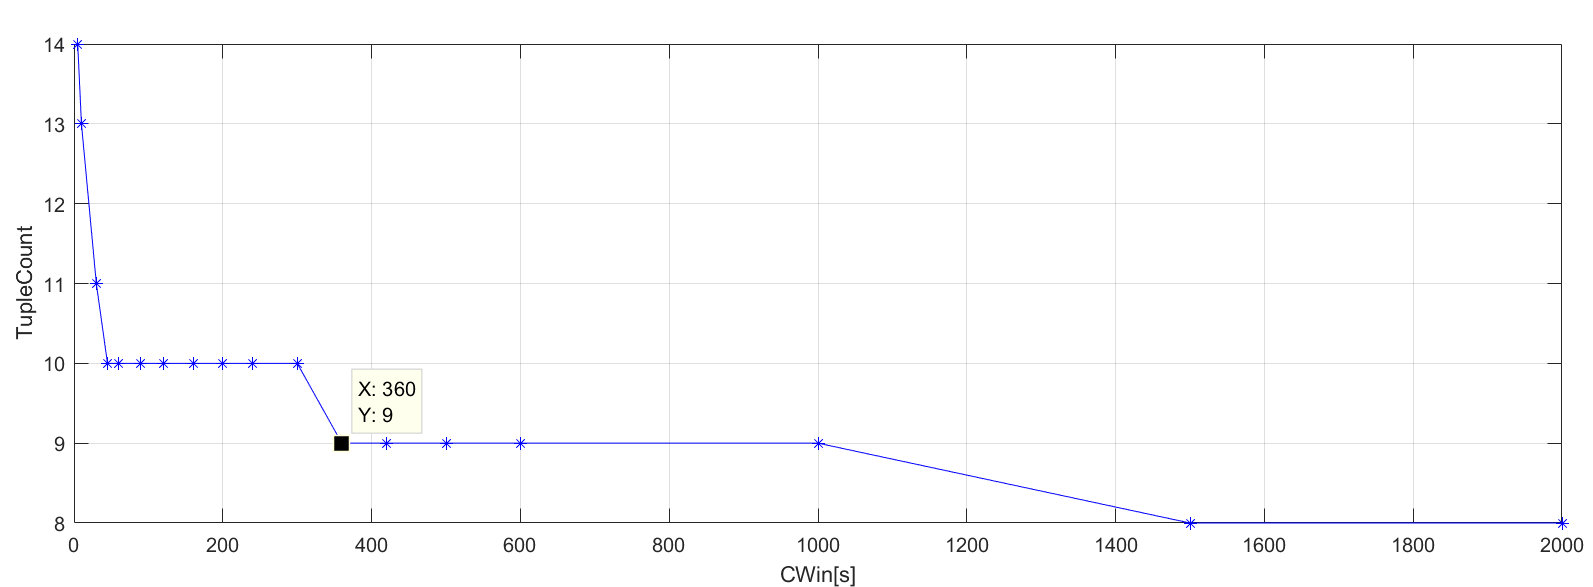
\includegraphics[width=\linewidth]{plot_tg_s044_cwin}
      \caption*{tg s044}
    \end{figure}
  \end{minipage}
  \begin{minipage}{0.49\linewidth}
    \hspace{0.25\linewidth}
    \begin{figure}[H]
      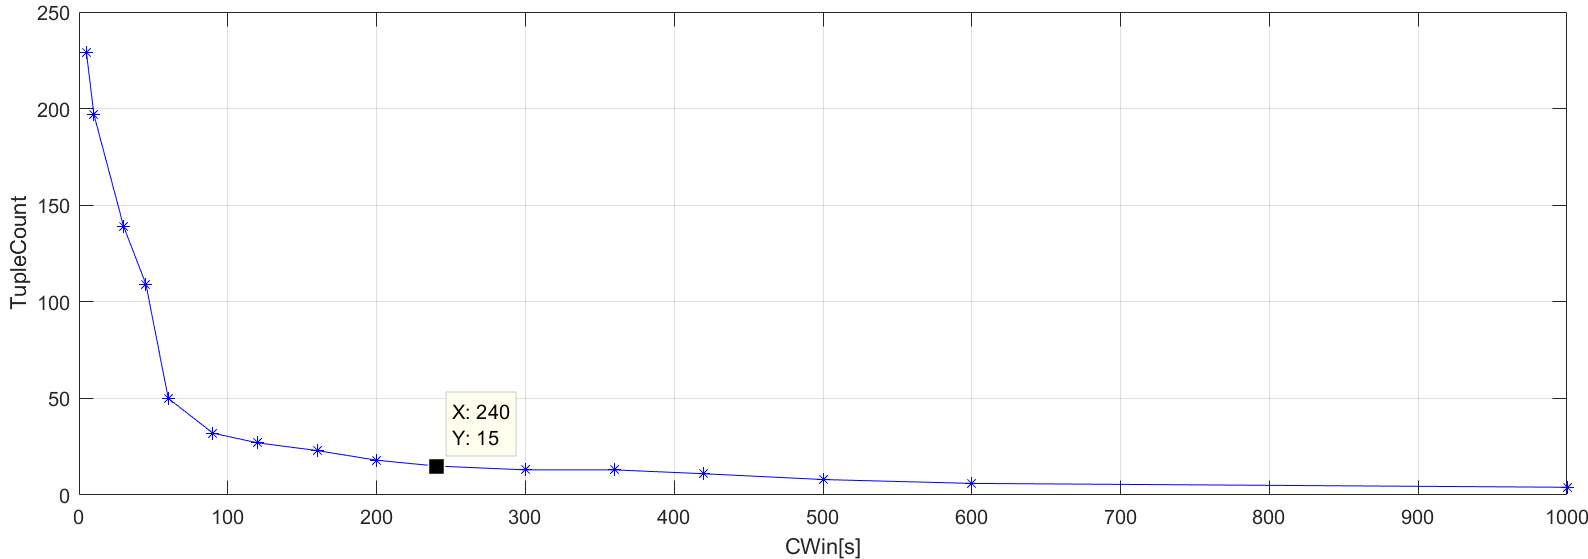
\includegraphics[width=\linewidth]{plot_tg_c238_cwin}
      \caption*{tg c238}
    \end{figure}
  \end{minipage}
\end{minipage}
\captionof{figure}{CWIN: log filtrato per Nodo}
\label{cwin_5_nodi}

\clearpage

Dalla seguente tabella si osserva che non è possibile scegliere un
valore univoco di finestra di coalescenza per tutti i nodi considerati, in quanto
i valori differiscono eccessivamente tra di loro.\\
Imponendo un unico valore di CWIN si potrebbe incorrere in problematiche di
collisioni tra differenti eventi di fallimento.\\

\begin{figure}[!htbp]
  \centering
  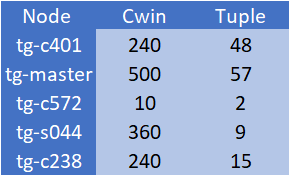
\includegraphics[width=.4\linewidth,keepaspectratio]{node_cwin}
\end{figure}

In seguito è riportato il confronto tra la reliability del sistema e quella dei
nodi che, fissato il valore CWIN, presentano più di 30 tuple.\\

\begin{minipage}{\linewidth}
  \centering
  \begin{minipage}{.49\linewidth}
    \begin{figure}[H]
      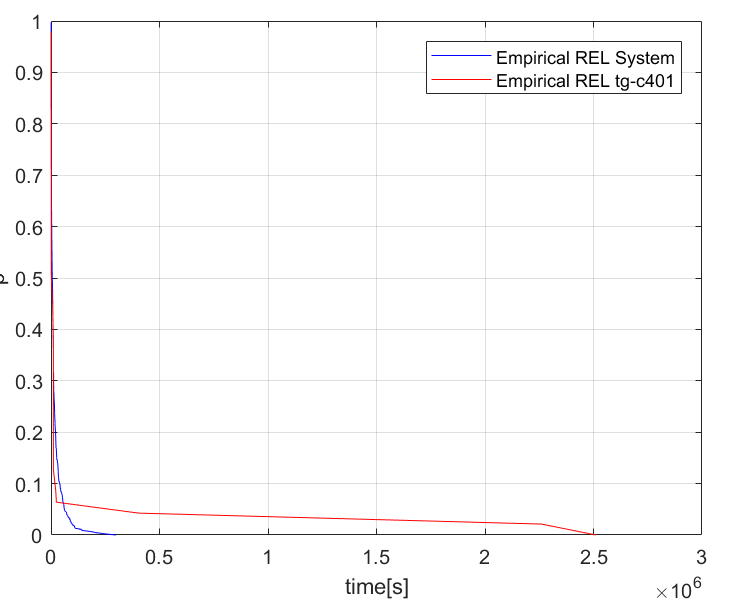
\includegraphics[width=\linewidth]{plot_rel_mercury_tg_c401}
      \caption*{tg c401}
    \end{figure}
  \end{minipage}
  \begin{minipage}{.49\linewidth}
    \begin{figure}[H]
      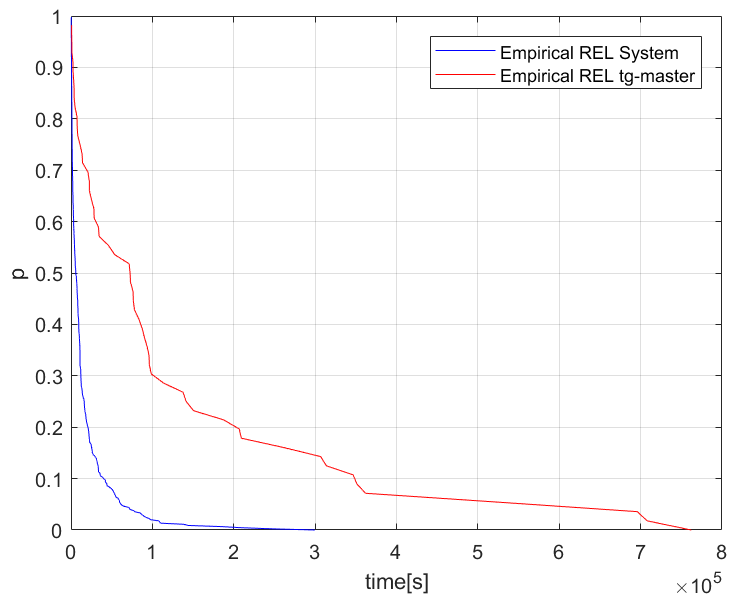
\includegraphics[width=\linewidth]{plot_rel_mercury_tg_master}
      \caption*{master}
    \end{figure}
  \end{minipage}
\end{minipage}
\captionof{figure}{Confronto Reliability Sistema e Nodi}

\clearpage

\subsection{Domanda 2}
\textit{Per ogni categoria di errore(escluso OTH), determinare CWIN, tuple count
ed il modello di reliability.
Inoltre, quale categoria è la pìù/meno Reliable?}

\subsubsection*{Soluzione}
Per poter rispondere alla domanda è necessario calcolare la finestra di coalescenza
per ogni log filtrato per categoria di errore.\\
I valori di CWIN ottenuti sono riportati in figura \ref{cwin_categorie}.\\

\begin{minipage}{\linewidth}
  \centering
  \begin{minipage}{0.49\linewidth}
    \begin{figure}[H]
      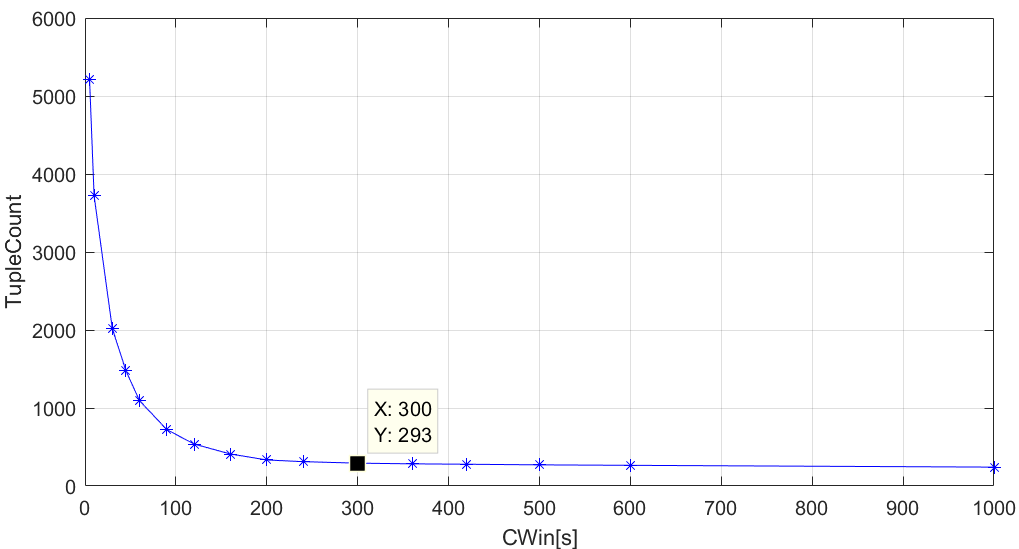
\includegraphics[width=\linewidth]{plot_CWIN_DEV}
      \caption*{dev}
    \end{figure}
  \end{minipage}
  \begin{minipage}{0.49\linewidth}
    \begin{figure}[H]
      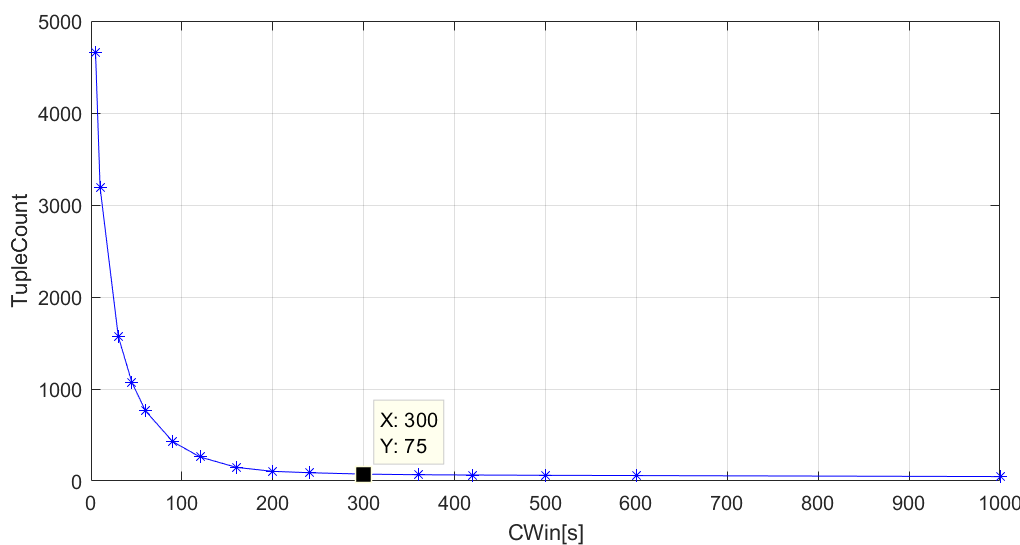
\includegraphics[width=\linewidth]{plot_CWIN_MEM}
      \caption*{mem}
    \end{figure}
  \end{minipage}
  \begin{minipage}{0.49\linewidth}
    \begin{figure}[H]
      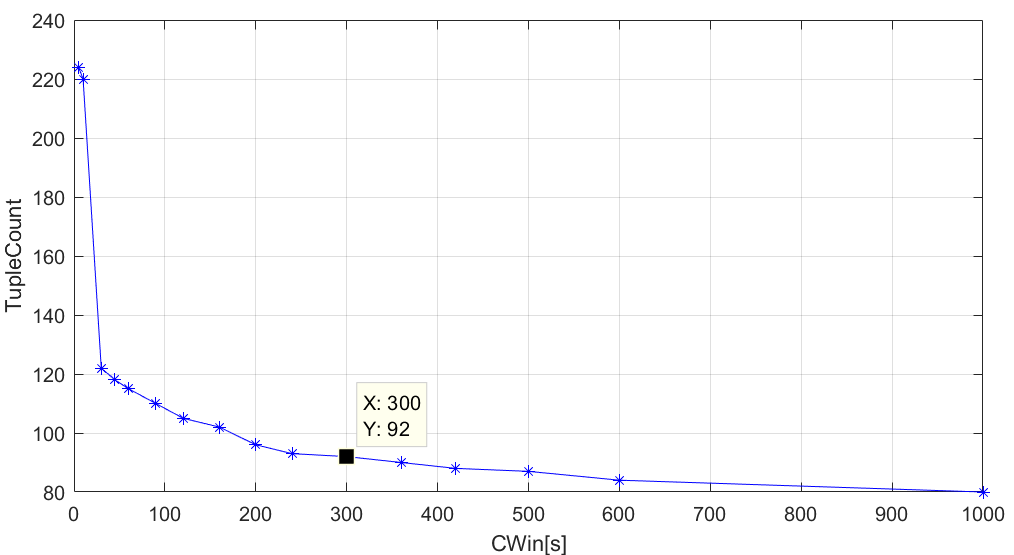
\includegraphics[width=\linewidth]{plot_CWIN_IO}
      \caption*{io}
    \end{figure}
  \end{minipage}
  \begin{minipage}{0.49\linewidth}
    \begin{figure}[H]
      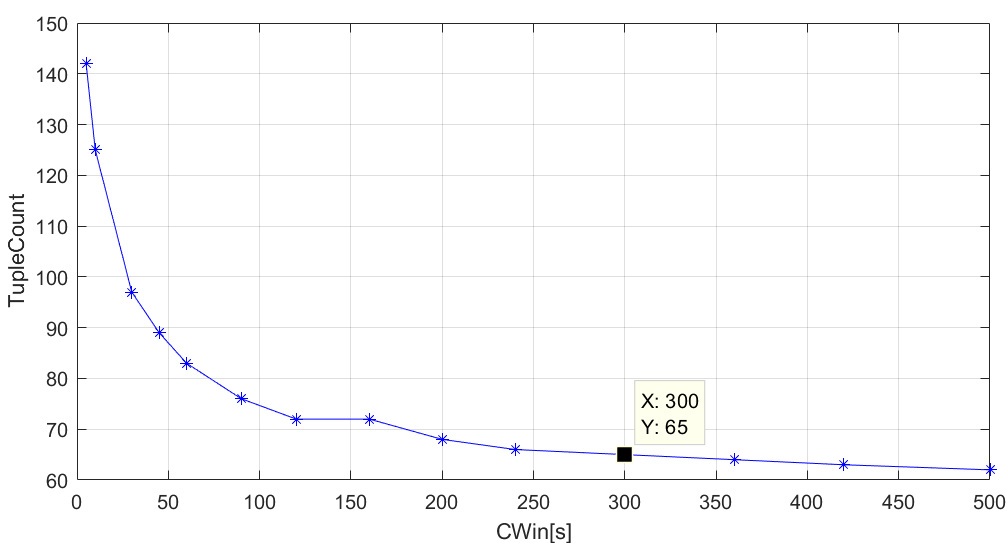
\includegraphics[width=\linewidth]{plot_CWIN_NET}
      \caption*{net}
    \end{figure}
  \end{minipage}
  \begin{minipage}{0.49\linewidth}
    \hspace{0.25\linewidth}
    \begin{figure}[H]
      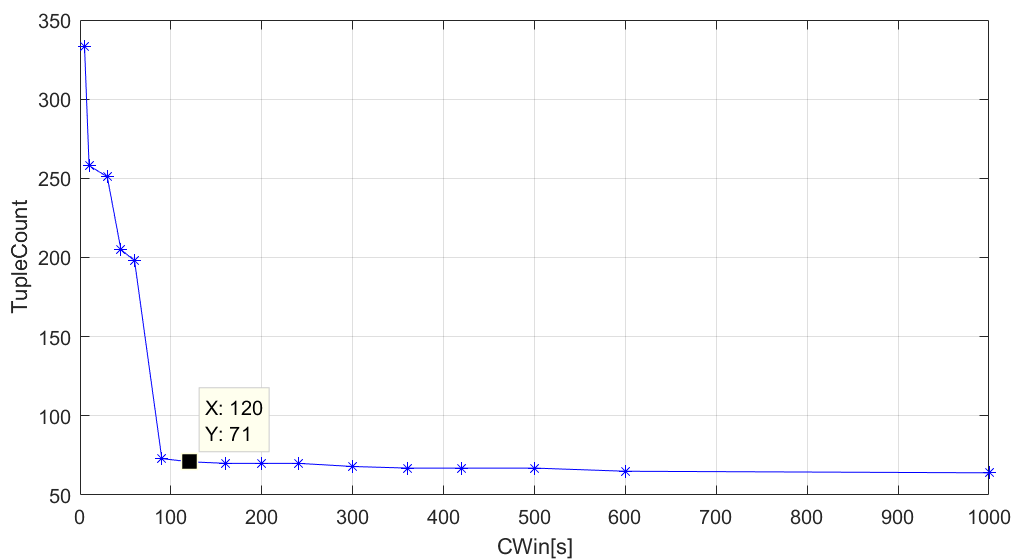
\includegraphics[width=\linewidth]{plot_CWIN_PRO}
      \caption*{pro}
    \end{figure}
  \end{minipage}
\end{minipage}
\captionof{figure}{CWIN: log filtrato per categoria di errore}
\label{cwin_categorie}

\clearpage

Il conteggio di tuple, divise in funzione delle categorie di errore, sono i
seguenti:

\begin{figure}[!htbp]
  \centering
  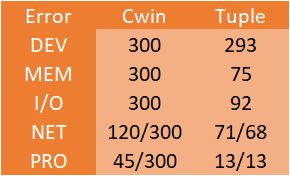
\includegraphics[width=.4\linewidth,keepaspectratio]{error_cwin}
  \caption{CWIN: log filtrato per categoria errore}
  \label{error_cwin}
\end{figure}

\clearpage

Le reliability empiriche, invece, sono riportati in figura \ref{modello_reliability_e}.\\

\begin{minipage}{\linewidth}
  \centering
  \begin{minipage}{0.49\linewidth}
    \begin{figure}[H]
      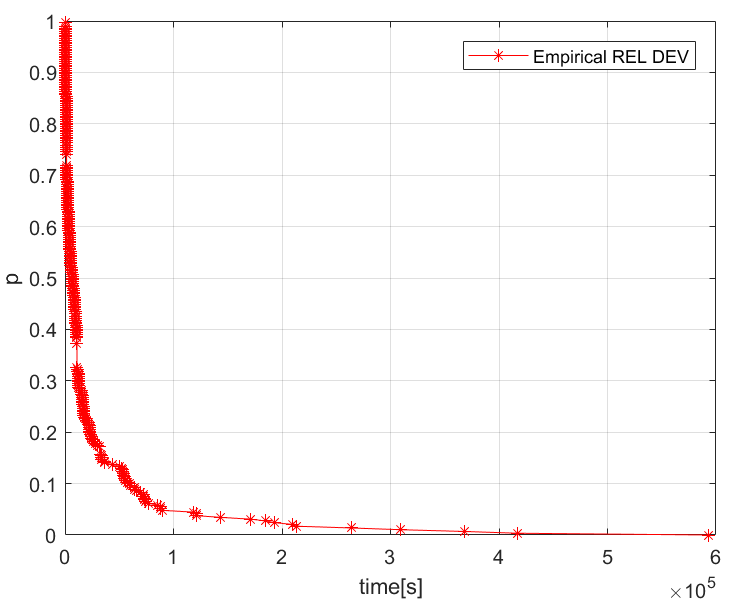
\includegraphics[width=.9\linewidth]{plot_reliability_DEV}
      \caption*{dev}
    \end{figure}
  \end{minipage}
  \begin{minipage}{0.49\linewidth}
    \begin{figure}[H]
      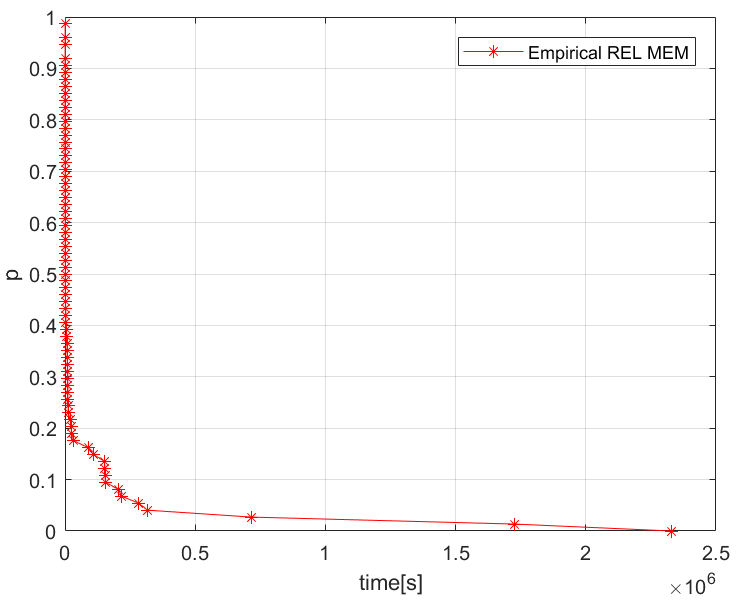
\includegraphics[width=.9\linewidth]{plot_reliability_MEM}
      \caption*{mem}
    \end{figure}
  \end{minipage}
  \begin{minipage}{0.49\linewidth}
    \begin{figure}[H]
      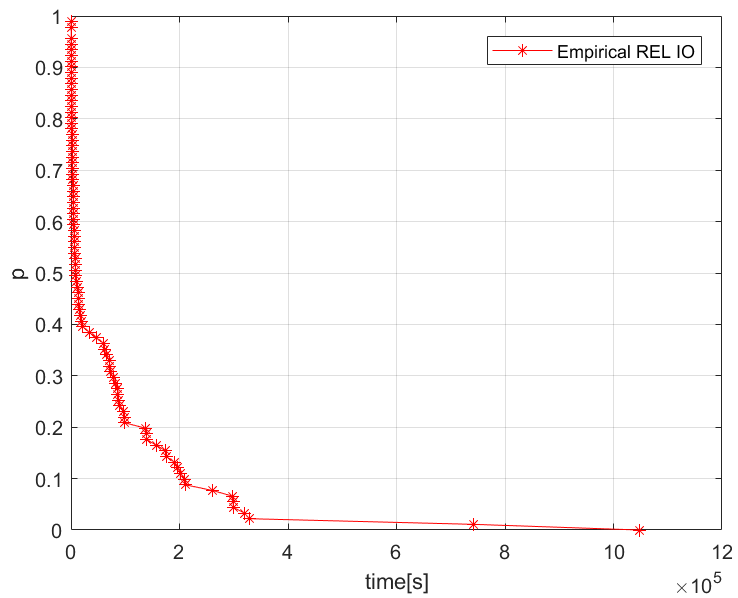
\includegraphics[width=.9\linewidth]{plot_reliability_IO}
      \caption*{io}
    \end{figure}
  \end{minipage}
  \begin{minipage}{0.49\linewidth}
    \begin{figure}[H]
      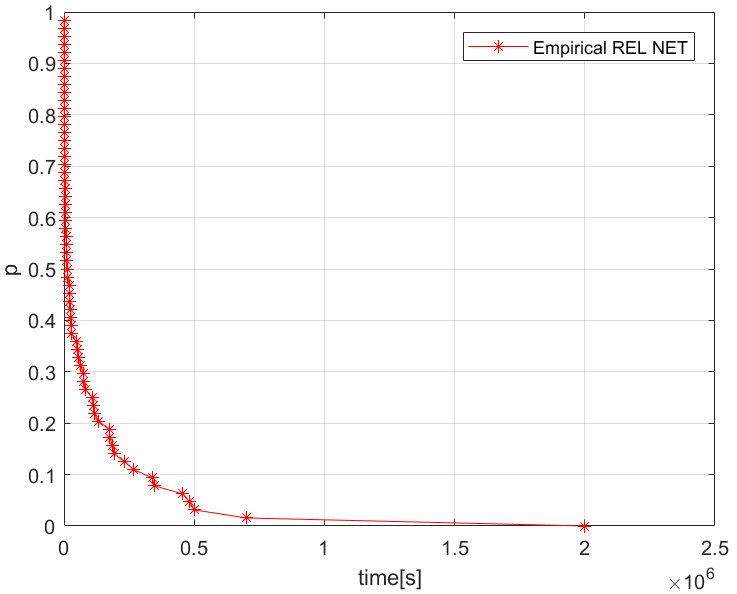
\includegraphics[width=.9\linewidth]{plot_reliability_NET}
      \caption*{net}
    \end{figure}
  \end{minipage}
  \begin{minipage}{0.49\linewidth}
    \hspace{0.25\linewidth}
    \begin{figure}[H]
      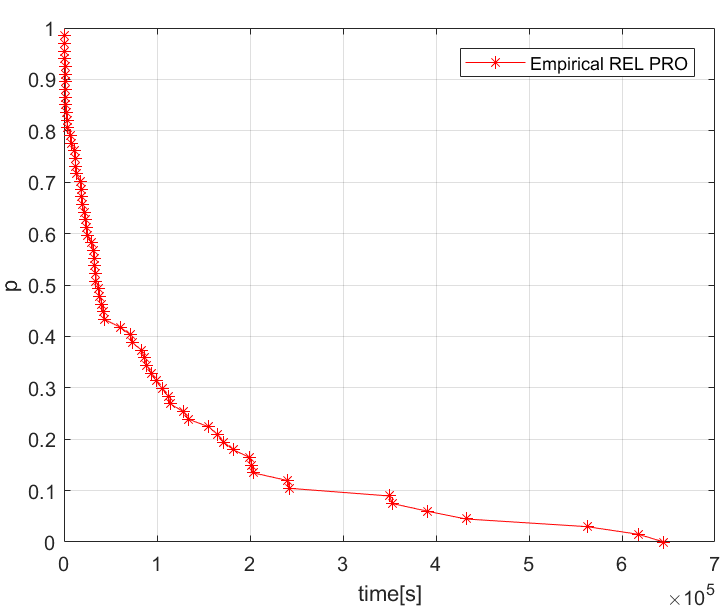
\includegraphics[width=.9\linewidth]{plot_reliability_PRO}
      \caption*{pro}
    \end{figure}
  \end{minipage}
\end{minipage}
\captionof{figure}{Reliability empirica}
\label{modello_reliability_e}

\clearpage

\subsubsection*{Reliability Model - DEV}

\begin{figure}[!htbp]
  \centering
  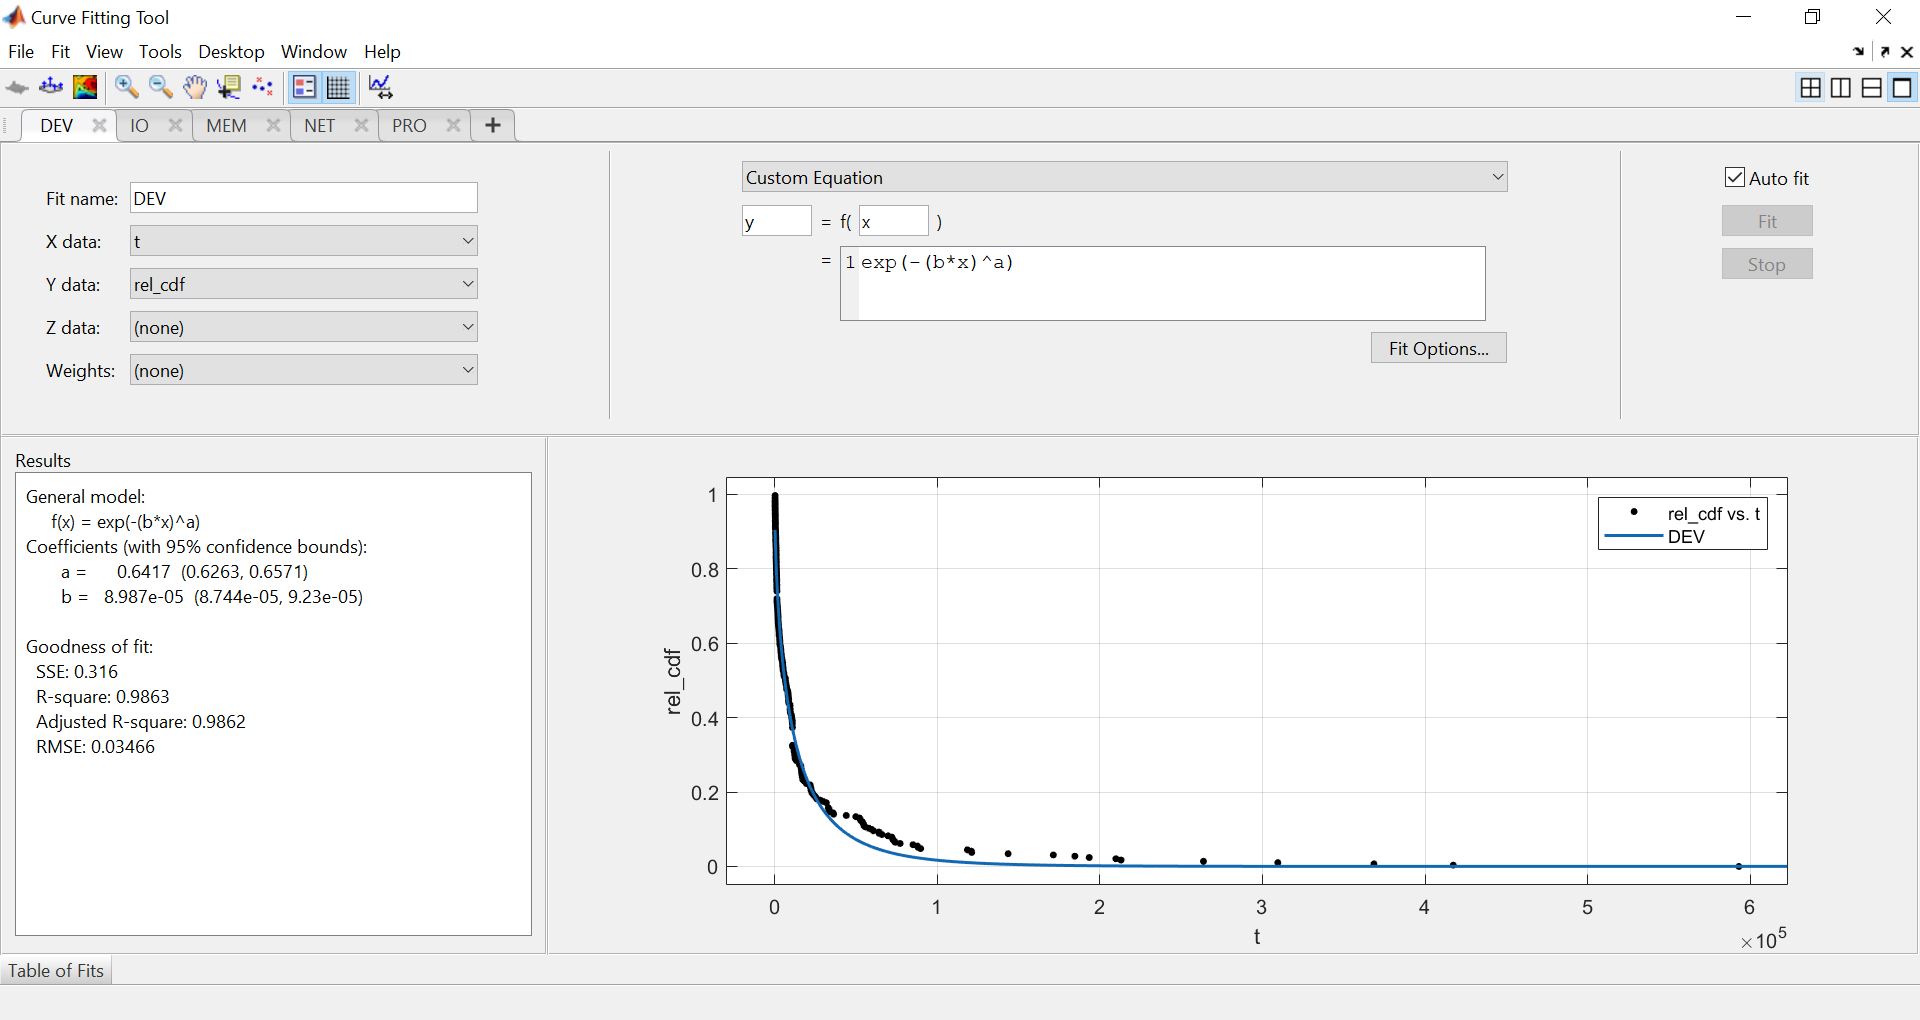
\includegraphics[width=0.9\linewidth,keepaspectratio]{rel_model_dev}
  \caption{Curve Fitting modello Weibull categoria di errore DEV}
  \label{rel_model_dev}
\end{figure}

Per valutare la bontà del fitting è stato utilizzato il \textbf{Kolmogorov-Smirnov Test}.\\

\begin{figure}[!htbp]
  \centering
  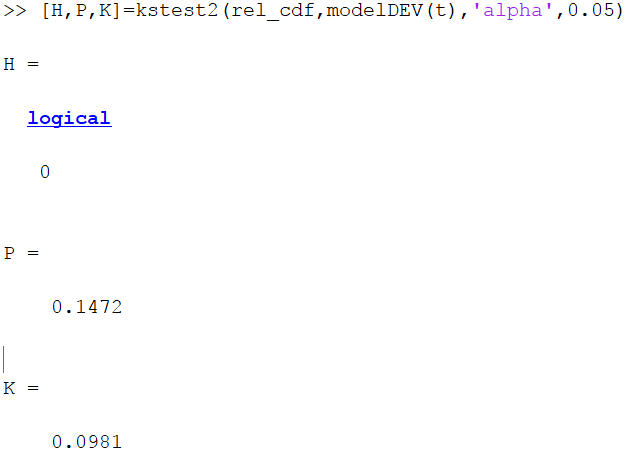
\includegraphics[width=0.5\linewidth,keepaspectratio]{ks_dev}
  \caption{Kolmogorov-Smirnov Test Weibull categoria di errore DEV}
  \label{ks_dev}
\end{figure}

L'ipotesi è rigettata con 85,28\% , con confidenza del 95\%.\\

\clearpage

\subsubsection*{Reliability Model - IO}

\begin{figure}[!htbp]
  \centering
  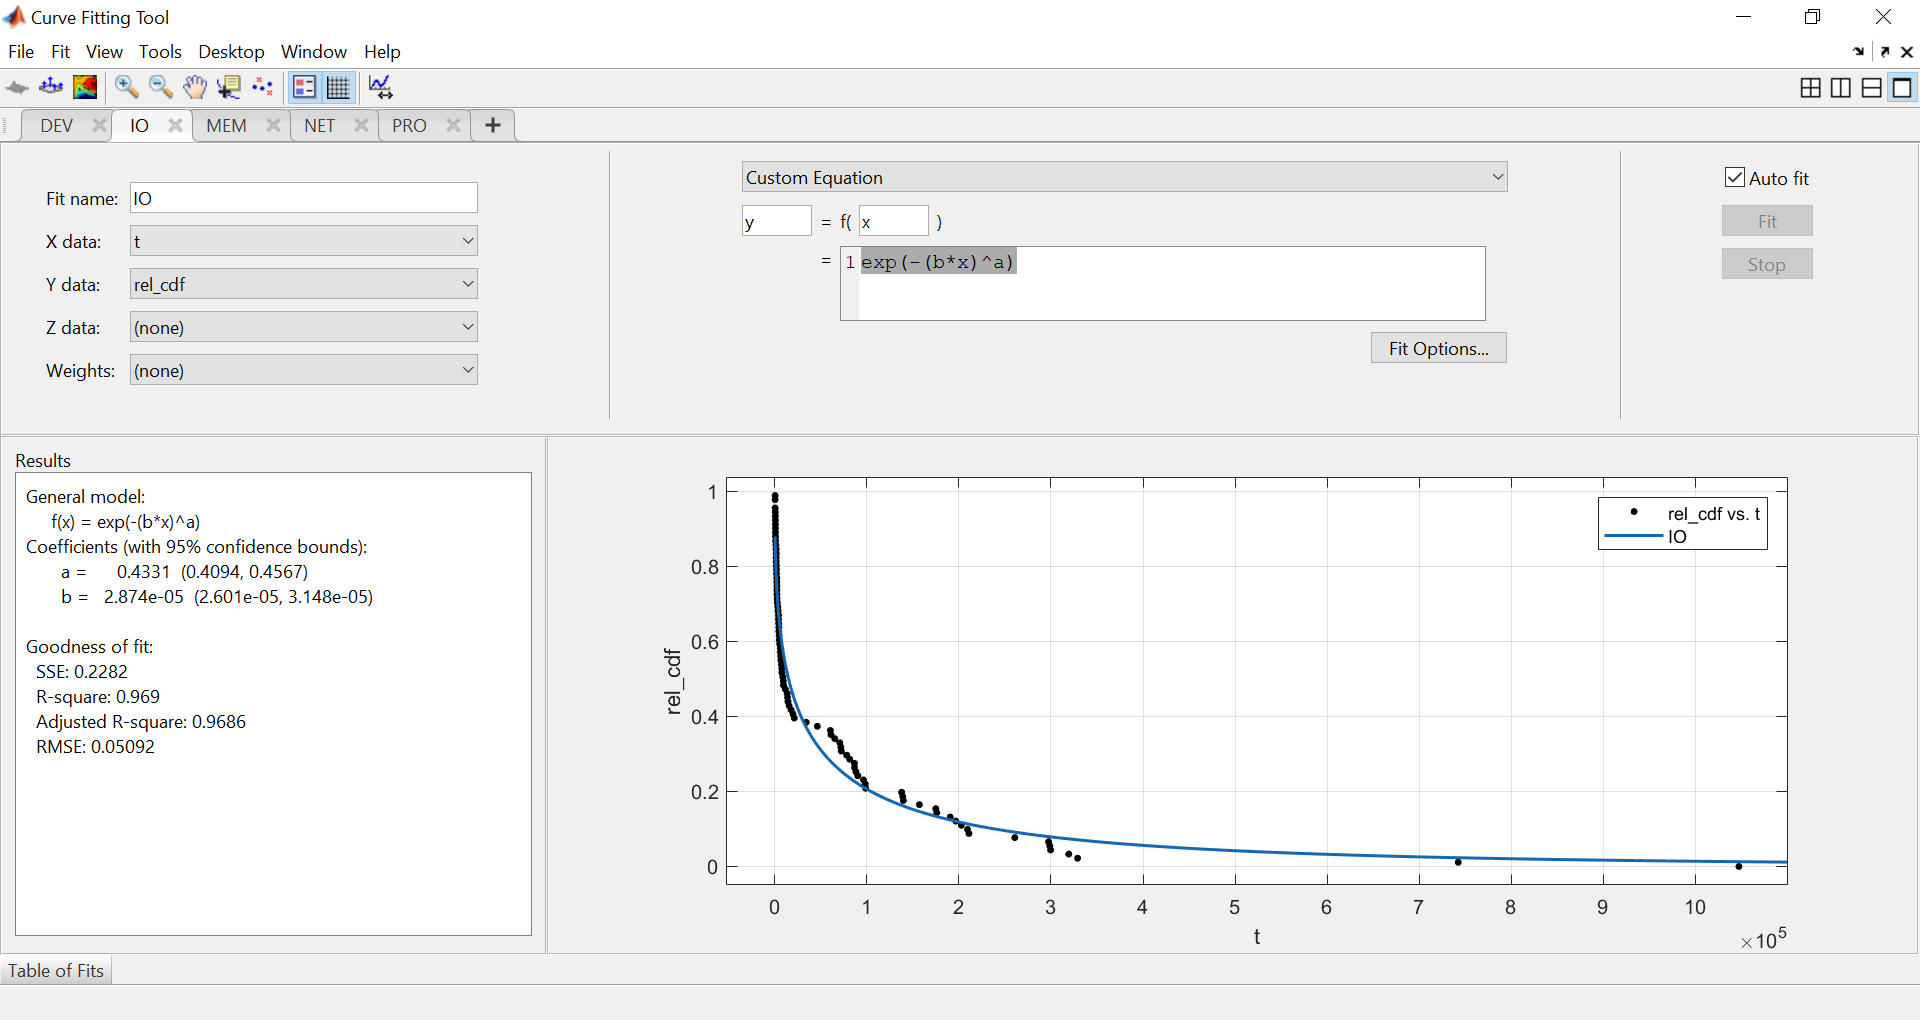
\includegraphics[width=0.9\linewidth,keepaspectratio]{rel_model_io}
  \caption{Curve Fitting modello Weibull categoria di errore IO}
  \label{rel_model_io}
\end{figure}

Per valutare la bontà del fitting è stato utilizzato il \textbf{Kolmogorov-Smirnov Test}.\\

\begin{figure}[!htbp]
  \centering
  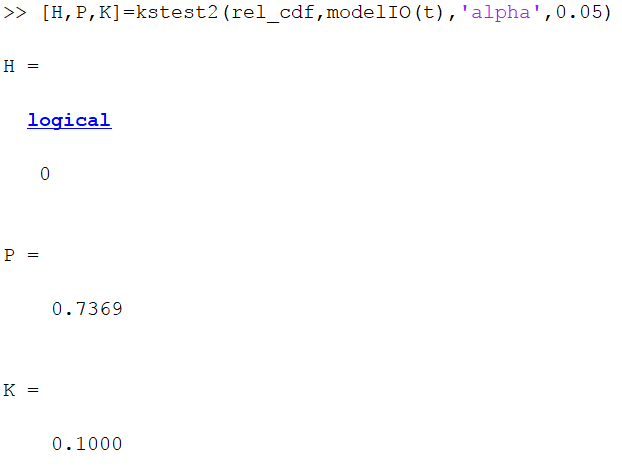
\includegraphics[width=0.5\linewidth,keepaspectratio]{ks_io}
  \caption{Kolmogorov-Smirnov Test Weibull categoria di errore IO}
  \label{ks_io}
\end{figure}

L'ipotesi non è rigettata al 73,69\%, con confidenza del 95\%.\\

\clearpage
\subsubsection*{Reliability Model - MEM}

\begin{figure}[!htbp]
  \centering
  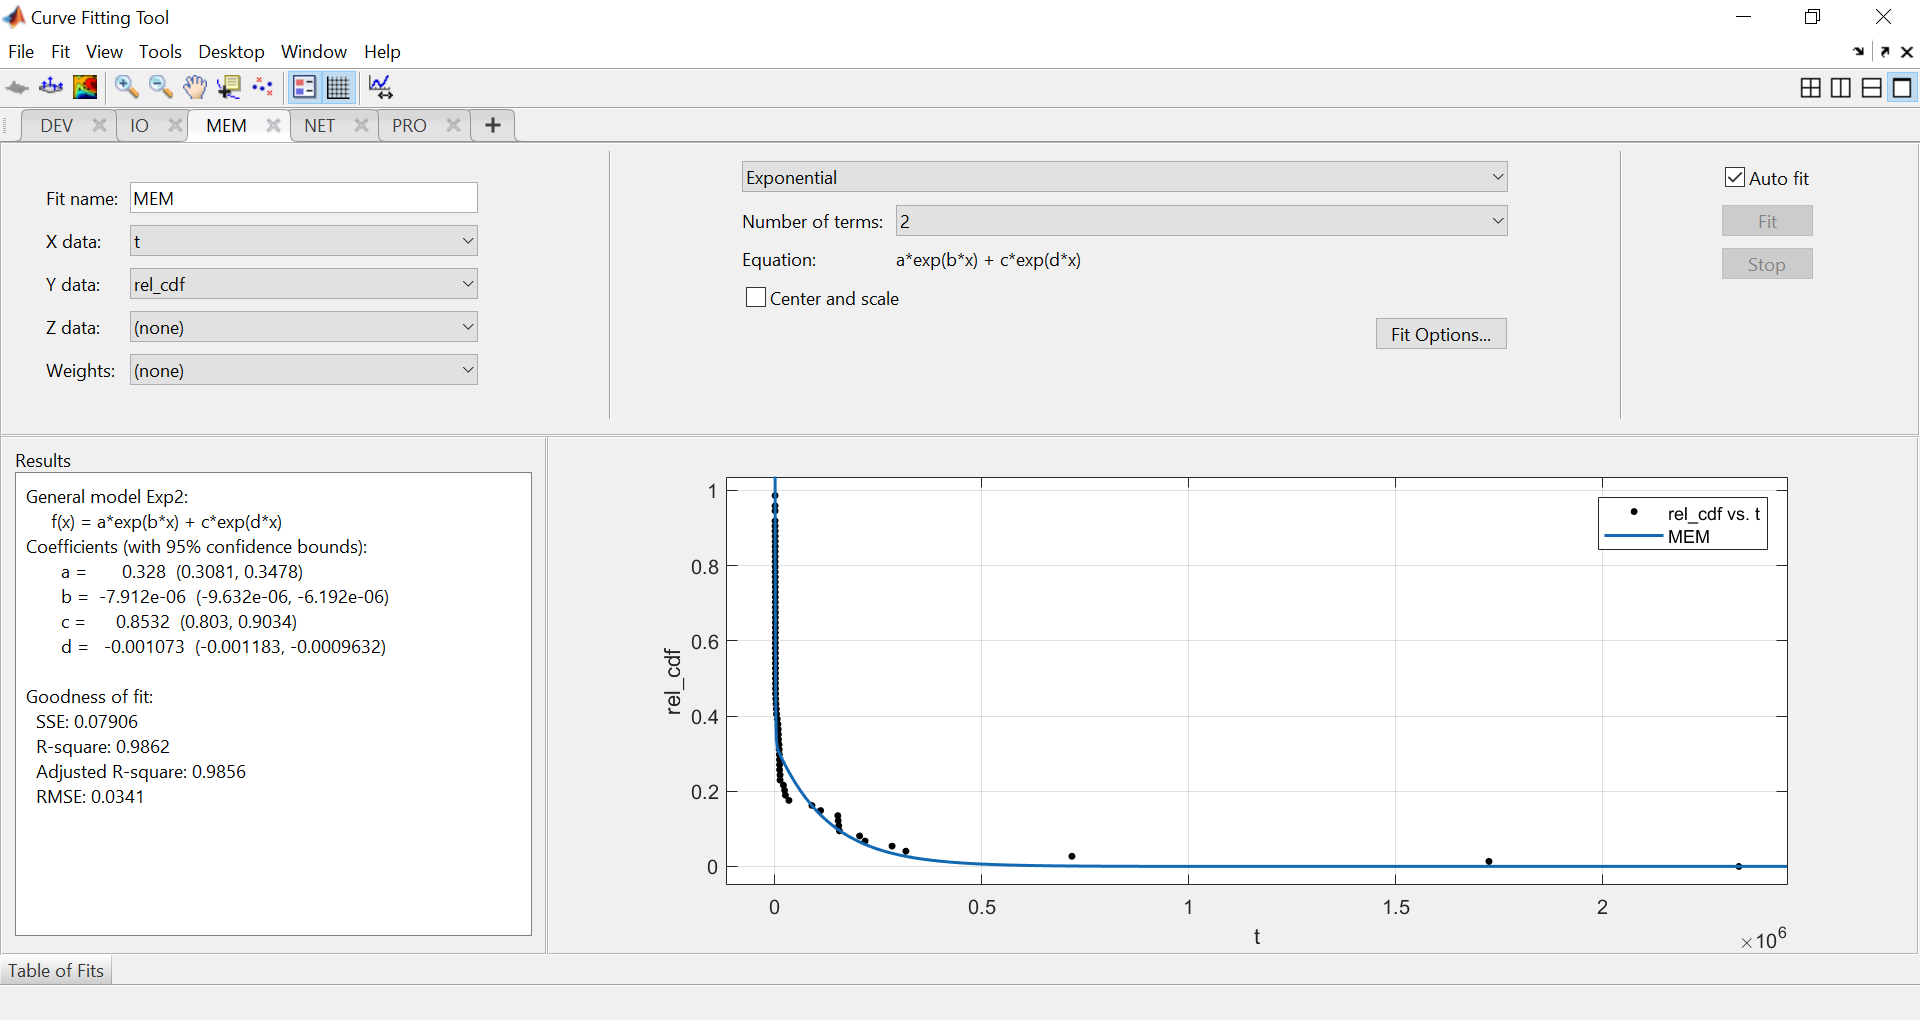
\includegraphics[width=0.9\linewidth,keepaspectratio]{rel_model_mem}
  \caption{Curve Fitting modello iperesponenziale categoria di errore MEM}
  \label{rel_model_mem}
\end{figure}

Per valutare la bontà del fitting è stato utilizzato il \textbf{Kolmogorov-Smirnov Test}.\\

\begin{figure}[!htbp]
  \centering
  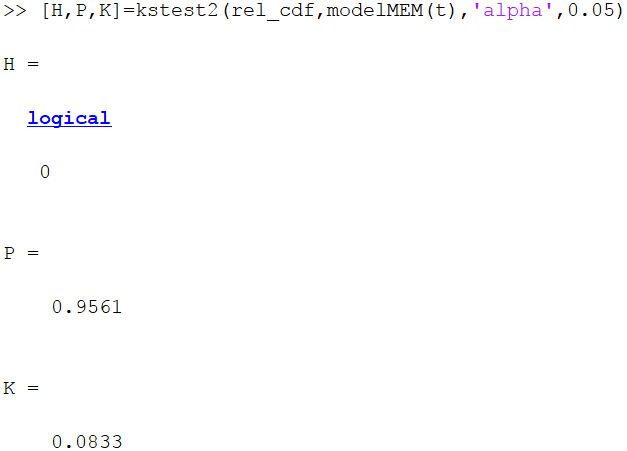
\includegraphics[width=0.5\linewidth,keepaspectratio]{ks_mem}
  \caption{Kolmogorov-Smirnov Test iperesponenziale categoria di errore MEM}
  \label{ks_mem}
\end{figure}

L'ipotesi non è rigettata al 95,61\% , con confidenza del 95\%.\\

\clearpage
\subsubsection*{Reliability Model - NET}

\begin{figure}[!htbp]
  \centering
  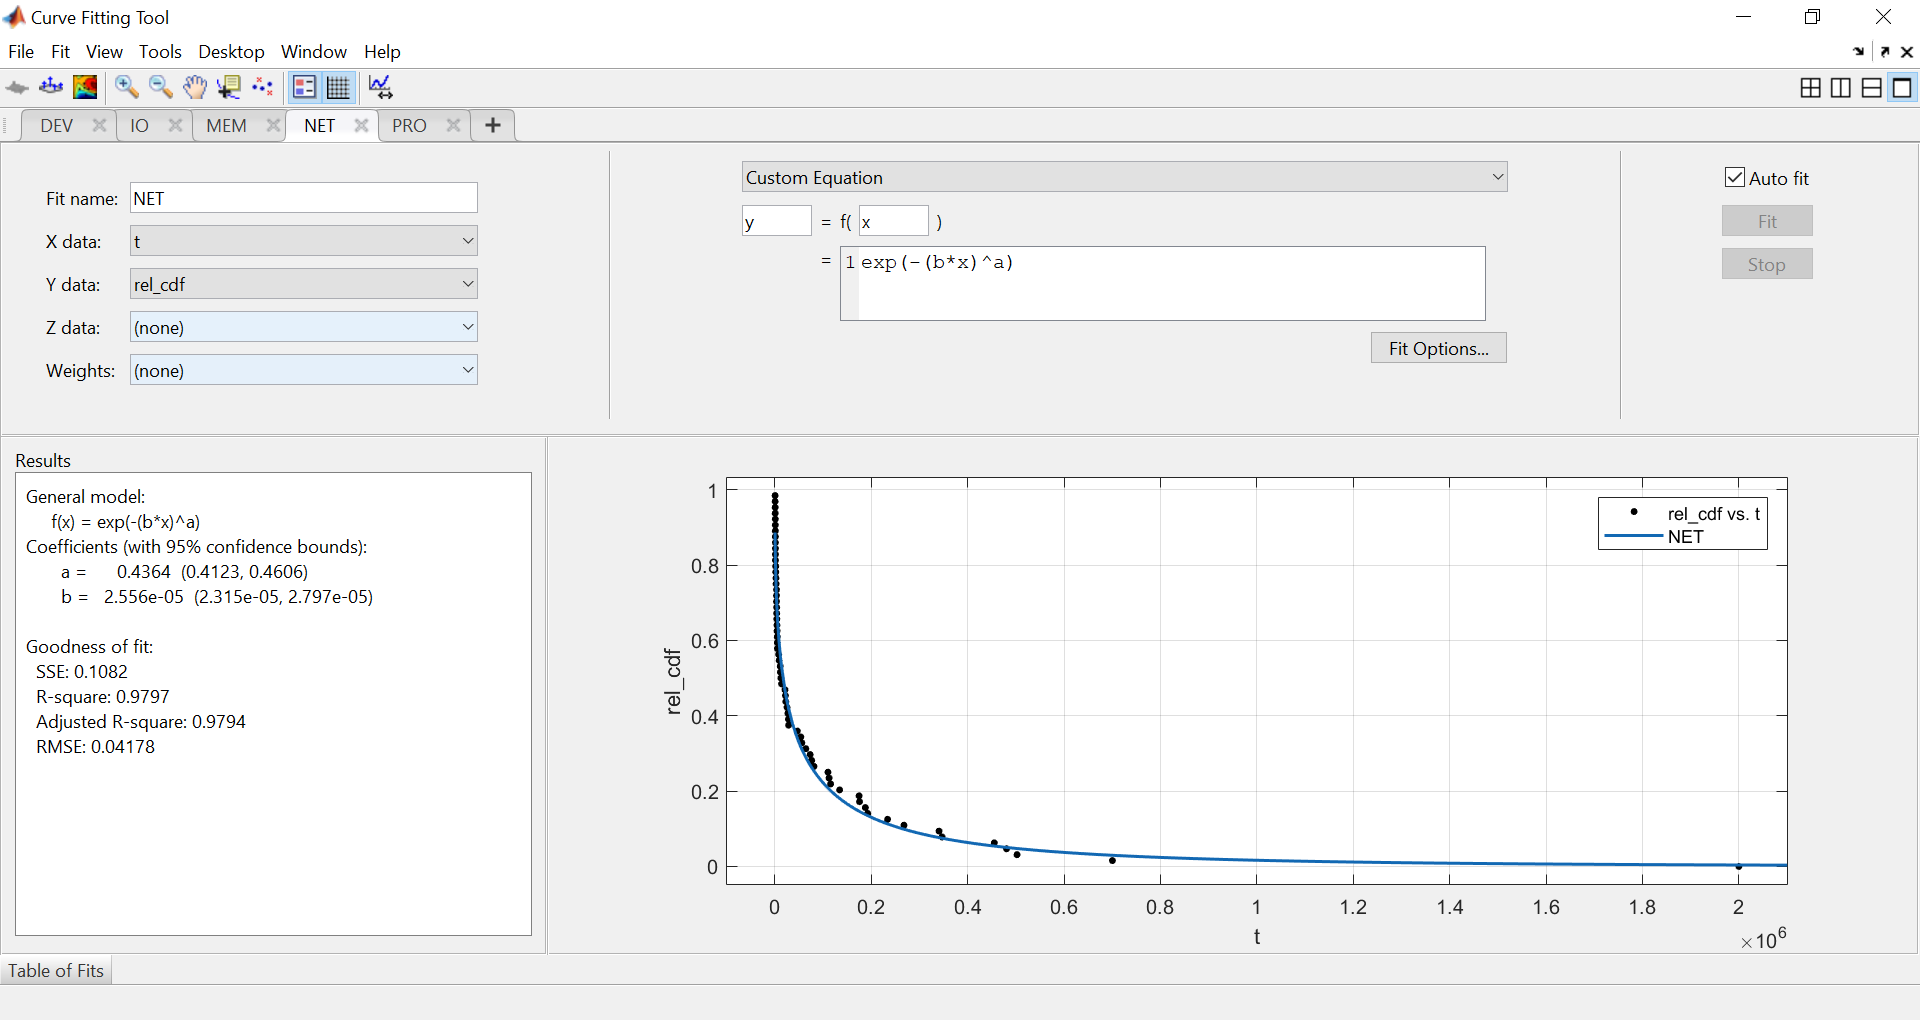
\includegraphics[width=0.9\linewidth,keepaspectratio]{rel_model_net}
  \caption{Curve Fitting modello Weibull categoria di errore NET}
  \label{rel_model_net}
\end{figure}

Per valutare la bontà del fitting è stato utilizzato il \textbf{Kolmogorov-Smirnov Test}.\\

\begin{figure}[!htbp]
  \centering
  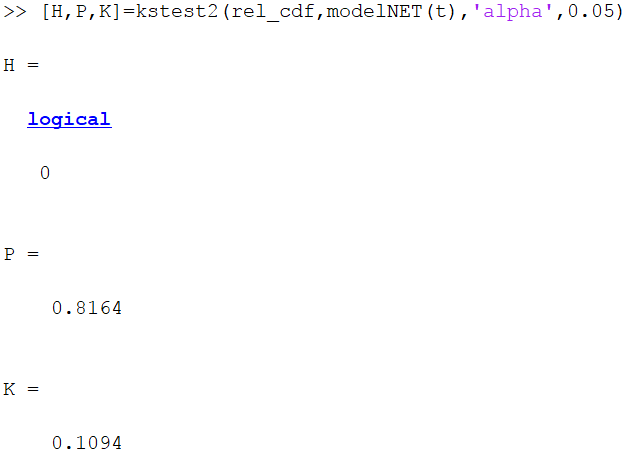
\includegraphics[width=0.5\linewidth,keepaspectratio]{ks_net}
  \caption{Kolmogorov-Smirnov Test Weibull categoria di errore NET}
  \label{ks_net}
\end{figure}

L'ipotesi non è rigettata al 81,64\%, con confidenza del 95\%.\\

\clearpage
\subsubsection*{Reliability Model - PRO}

\begin{figure}[!htbp]
  \centering
  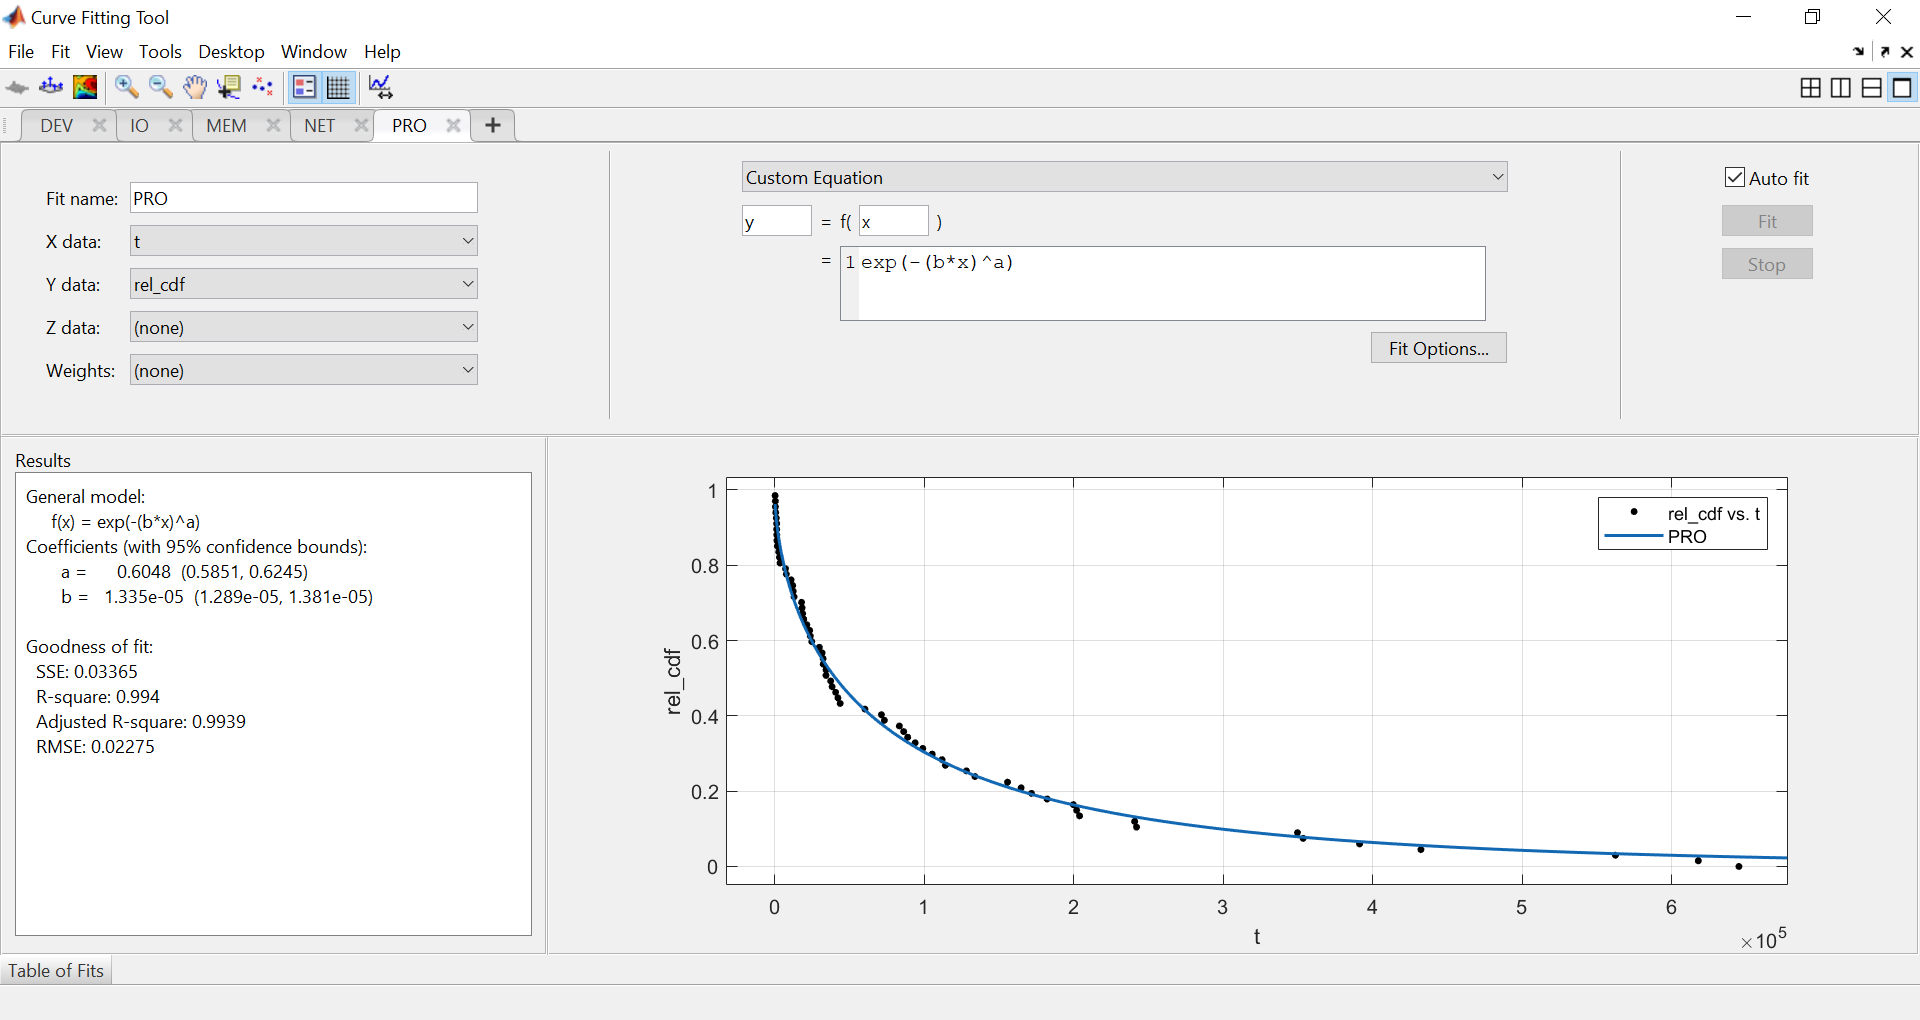
\includegraphics[width=0.9\linewidth,keepaspectratio]{rel_model_pro}
  \caption{Curve Fitting modello Weibull categoria di errore PRO}
  \label{rel_model_pro}
\end{figure}

Per valutare la bontà del fitting è stato utilizzato il \textbf{Kolmogorov-Smirnov Test}.\\

\begin{figure}[!htbp]
  \centering
  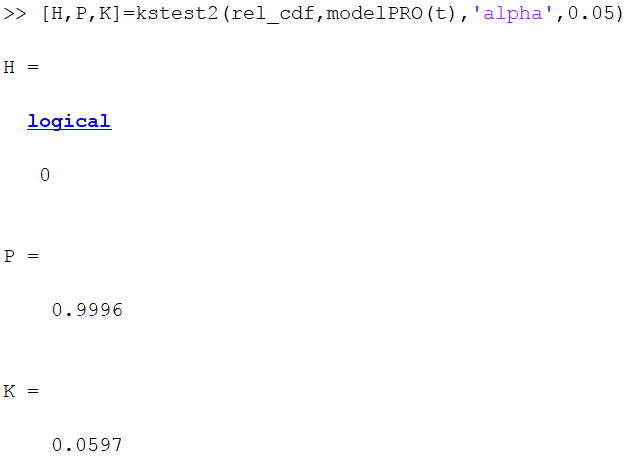
\includegraphics[width=0.5\linewidth,keepaspectratio]{ks_pro}
  \caption{Kolmogorov-Smirnov Test Weibull categoria di errore PRO}
  \label{ks_pro}
\end{figure}

L'ipotesi non è rigettata al 99,96\%, con confidenza del 95\%.\\

\clearpage

Studiando le figure \ref{error_cwin} e \ref{rel_models} è possibile osservare
che la categoria più reliable è \textit{PRO}(13), la meno è \textit{DEV}(293).\\

\begin{figure}[!htbp]
  \centering
  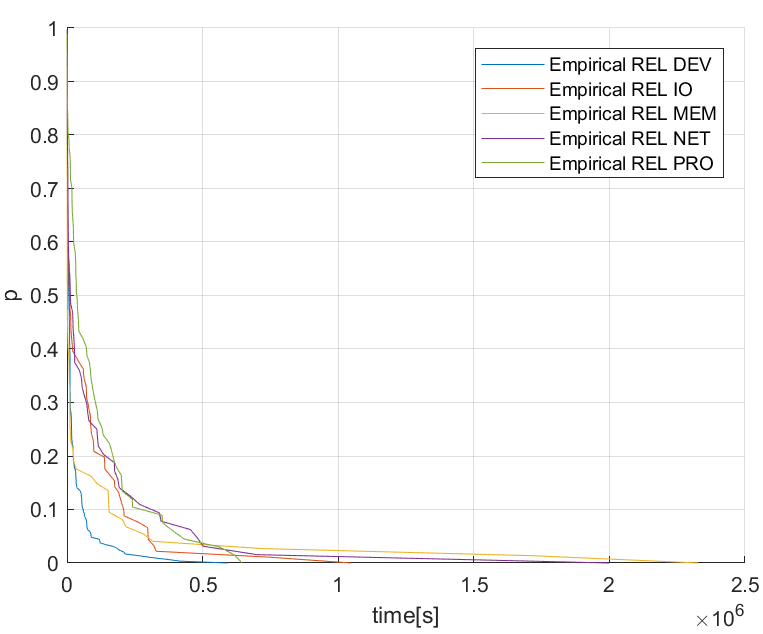
\includegraphics[width=\linewidth,keepaspectratio]{rel_conf_error}
  \caption{Confronto modelli di Reliability}
  \label{rel_models}
\end{figure}

\clearpage

\section{Blue Gene L}
Blue Gene L è un super-calcolatore IBM.\\
I nodi che compongono il sistema, riportati nel log, sono:
\begin{itemize}
  \item \textbf{Rack}: individuato nel log con la lettera R, seguita da un numero,
  rappresenta la cabina contenente i nodi;
  \item \textbf{Nodo}: individuato nel log con la lettera N, seguita da un numero,
  rappresenta, il blade del Rack contenente più Compute Card;
  \item \textbf{Compute Card}: individuata nel log con la lettera J, seguita da un
  numero compreso tra 1 e 16;
  \item \textbf{Compute Chip}: individuati nel log come U01 e U11, per ogni Compute
  Card ne sono presenti 2;
  \item \textbf{I-O Card}: individuata nel log come J18, è presente solo in alcuni
  nodi(N0,N4,N8,NC).
\end{itemize}

Il log è formato dai seguenti campi:
\begin{itemize}
  \item \textbf{Timestamp};
  \item \textbf{Nodo Origine};
  \item \textbf{Card Origine};
  \item \textbf{Messaggio}.
\end{itemize}

\clearpage

\subsection{Finestra di Coalescenza - CWIN}
La finestra di coalescenza, definita in secondi, definisce un intervallo temporale
in cui cadono tutti gli eventi che vi appartengono.\\
Lo script \textbf{tupleCount\_func\_CWINpy.sh}(riportato in figura \ref{coalescence_window_mercury}), con input i file \textit{MercuryErrorLog.txt}
e \textit{tentative-CWIN.txt}, è stato utilizzato per calcolare il numero di tuple al
variare della dimensione della finestra di coalescenza.\\

\begin{figure}[!htbp]
  \centering
  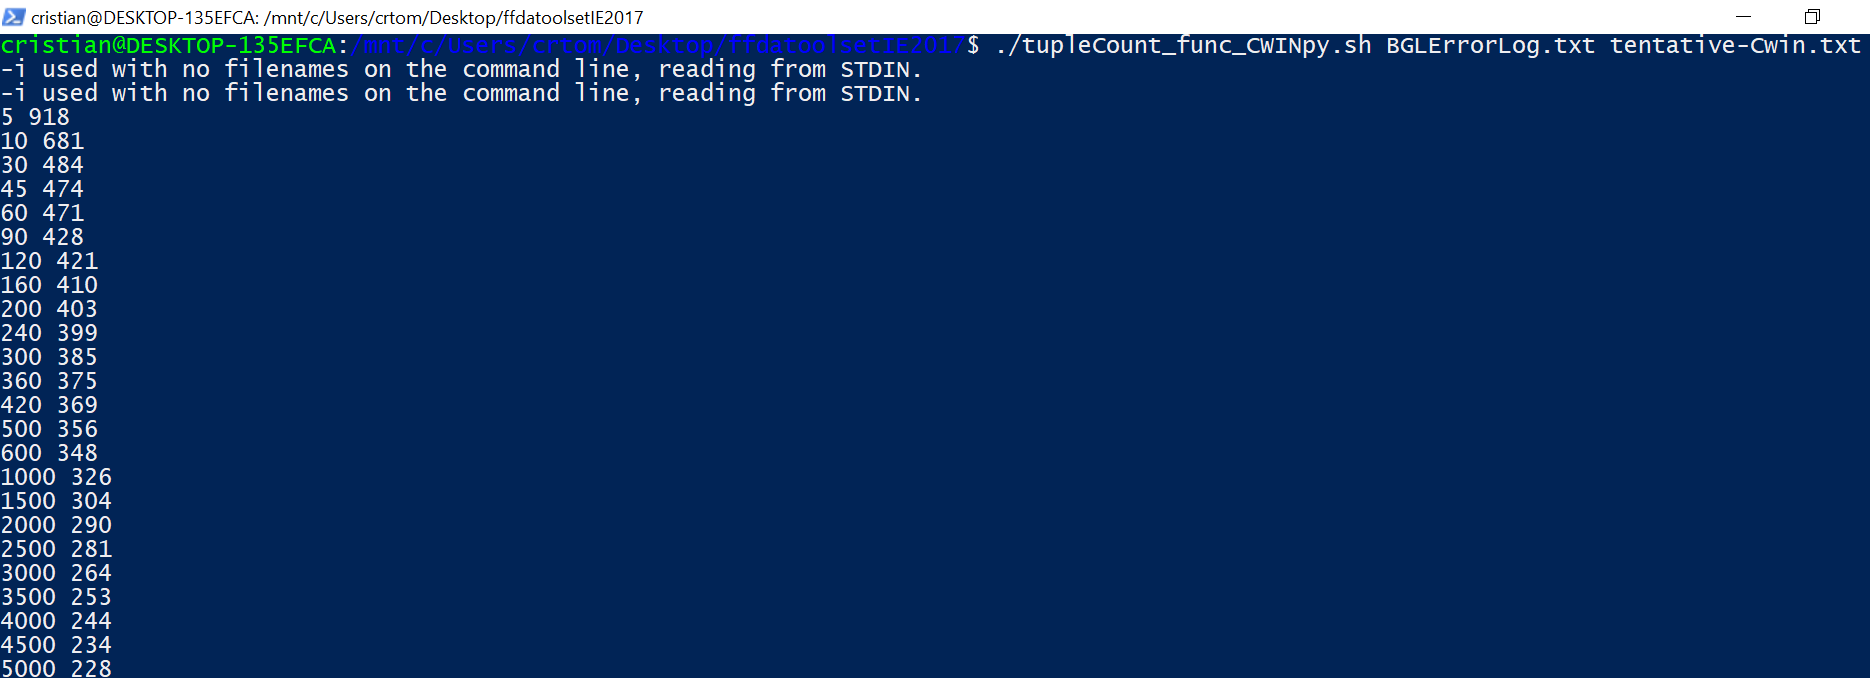
\includegraphics[width=1\linewidth,keepaspectratio]{coalescence_window_bgl}
  \caption{Script conteggio tuple al variare della finestra di coalescenza}
  \label{coalescence_window_bgl}
\end{figure}

L'output di tale script, plottato in matlab e presente in figura \ref{plot_coalescence_window_bgl},
è infine utilizzato per determinare un singolo valore di CWIN, ottenuto
considerando il punto successivo al ginocchio(knee) della curva.\\
Il valore di CWIN scelto è 500.\\
\begin{figure}[!htbp]
  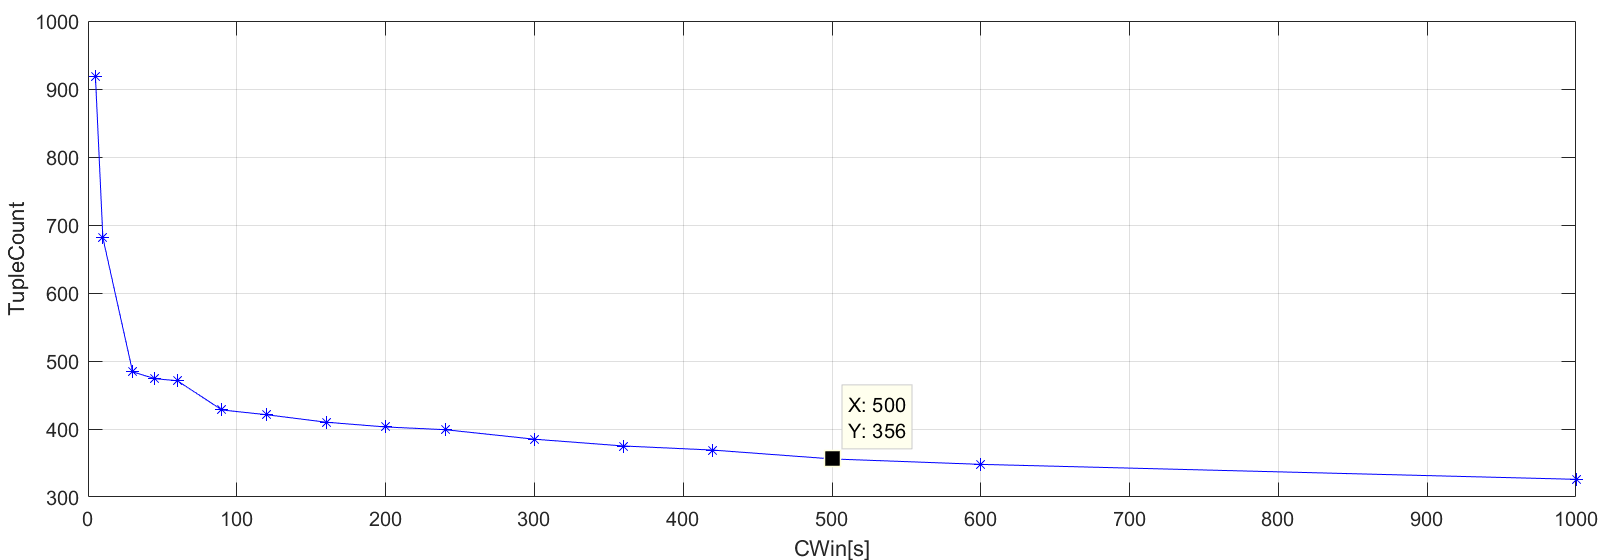
\includegraphics[width=1\linewidth,keepaspectratio]{plot_coalescence_window_bgl}
  \caption{Plot finestre di coalescenza}
  \label{plot_coalescence_window_bgl}
\end{figure}

Lo script bash \textbf{tupling\_with\_CWIN.sh} suddivide le righe del file di log,
in funzione del valore della finestra di coalescenza, raccogliendo, per ogni tupla,
le seguenti informazioni:

\begin{itemize}
  \item \textbf{Starting Points}: il timestamp della prima riga di ogni tupla generata;
  \item \textbf{Interarrivals}: il tempo che intercorre tra l'ultima riga e la
  prima riga di due tuple consecutive;
  \item \textbf{Lenghts}: il numero di righe presenti in ogni tupla.
\end{itemize}

Analizzando il file \textbf{interarrivals.txt} in matlab tramite lo script \textbf{ttf\_ref}
si ottiene la CDF empirica della TTF(Time To Failure) e dualmente la Reliability (1-TTF).\\
In figura è riportato il grafico delle due CDF.

\begin{figure}[!htbp]
  \centering
  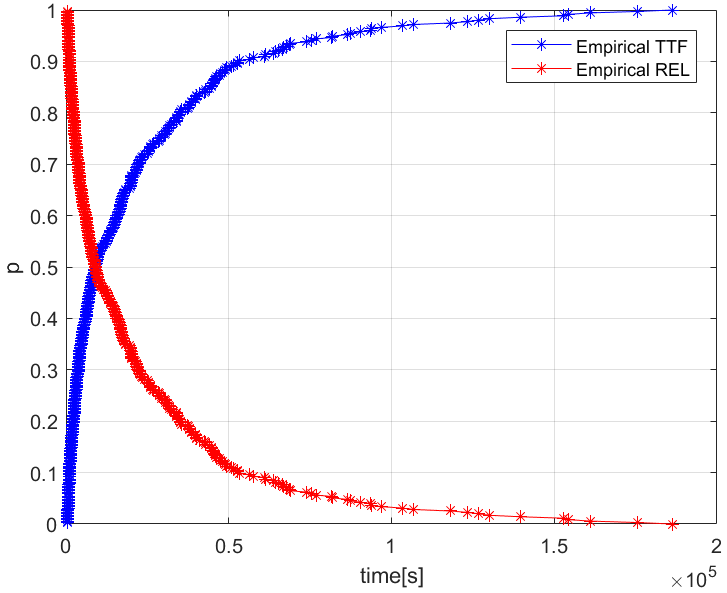
\includegraphics[width=.9\linewidth,keepaspectratio]{ttf_rel_bgl}
  \caption{Plot TTF e Reliability}
  \label{ttf_rel_bgl}
\end{figure}


\subsection{Curve Fitting}

Dopo aver ottenuto la CDF della reliability è possibile procedere con il fitting.\\
Utilizzando il tool di matlab \textbf{Curve Fitting} è stato possibile
analizzare i seguenti modelli:

\clearpage

\begin{itemize}
  \item \textbf{Esponenziale}:
  $$ y = e^{- \lambda  x} $$
  Il valore $\lambda$ è stato inizializzato a $1/MTTF$.\\
  Il modello risultante in matlab è riportato nella figura \ref{Exponential_bgl}.\\

  \begin{figure}[!htbp]
    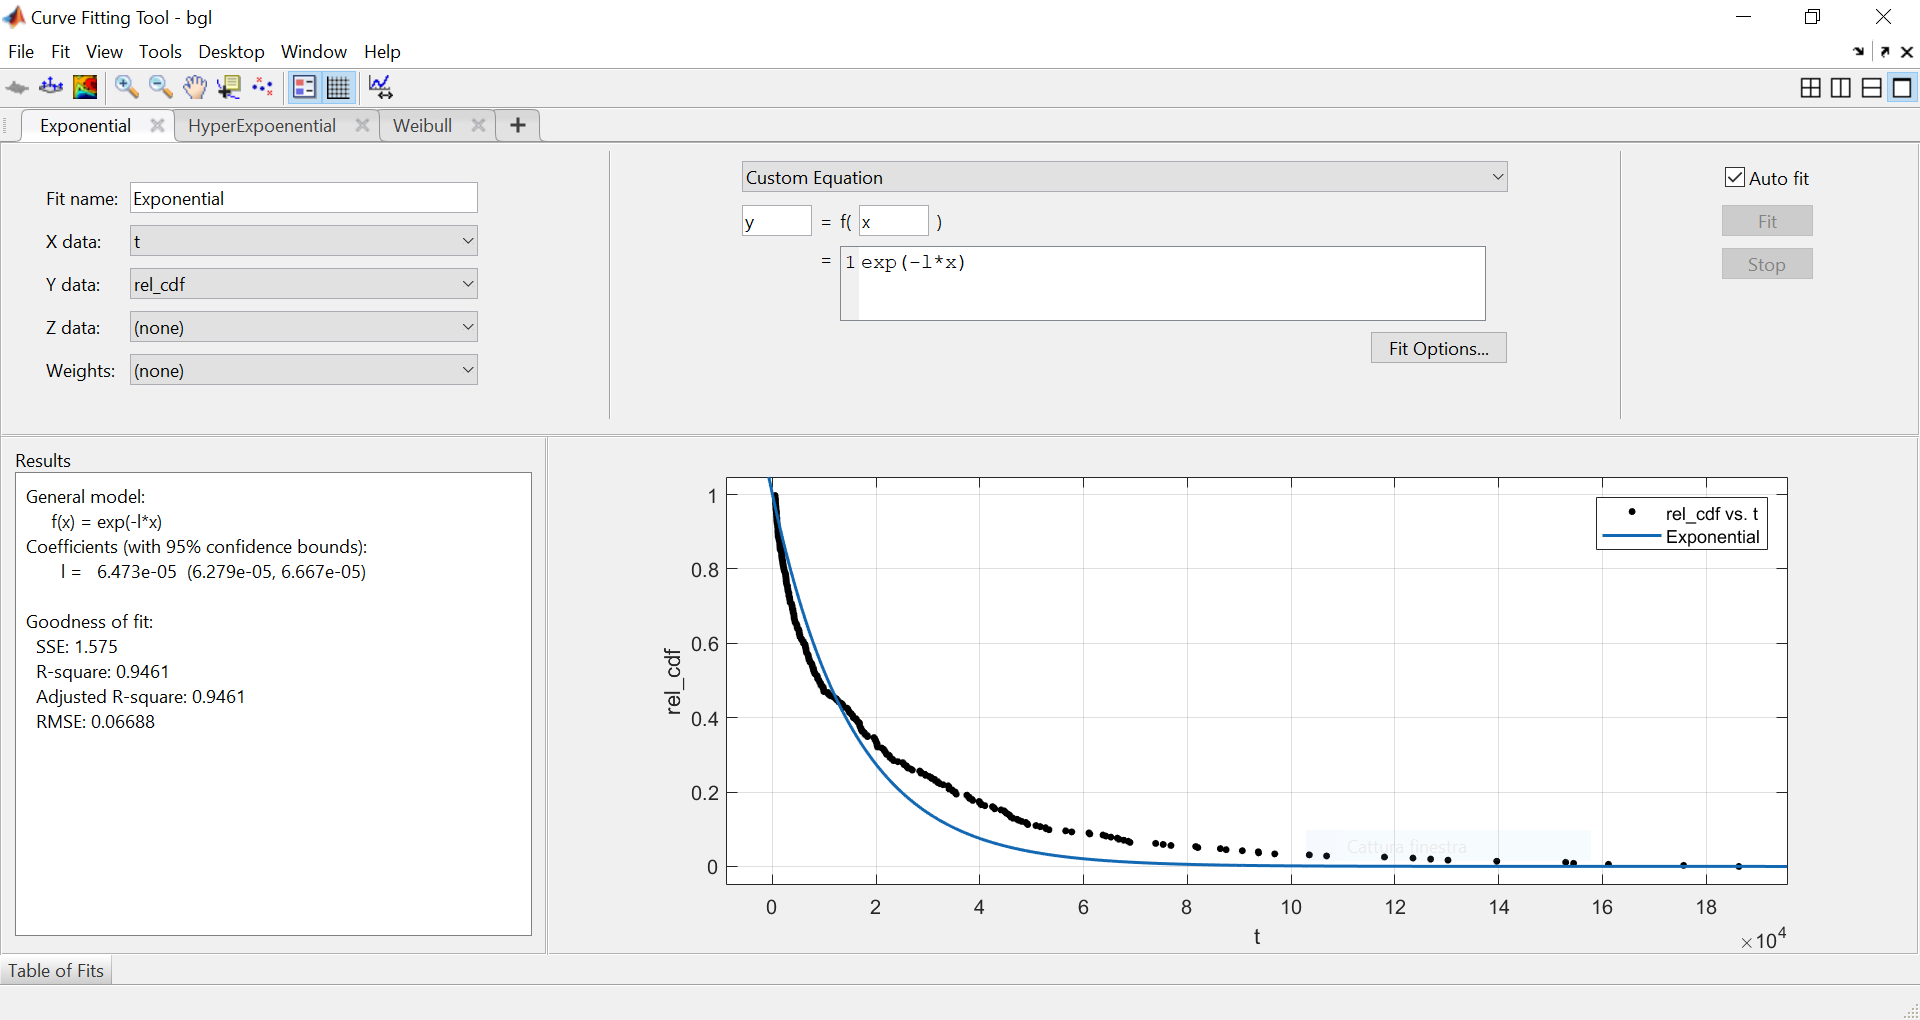
\includegraphics[width=.9\linewidth,keepaspectratio]{Exponential_bgl}
    \caption{Curve Fitting modello Esponenziale}
    \label{Exponential_bgl}
  \end{figure}

  Per valutare la bontà del fitting è stato utilizzato il \textbf{Kolmogorov-Smirnov Test}.\\

  \begin{figure}[!htbp]
    \centering
    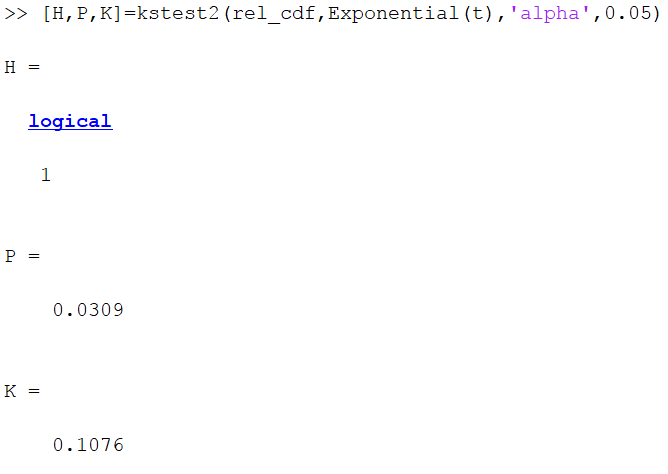
\includegraphics[width=0.5\linewidth,keepaspectratio]{ks_exp_bgl}
    \caption{Kolmogorov-Smirnov Test esponenziale}
    \label{ks_exp_bgl}
  \end{figure}

  L'ipotesi nulla è rigettata al 96,91\%, con confidenza del 95\%.

  \clearpage

  \item \textbf{Weibull}:
  $$ y = e^{- (\lambda x)^\alpha} $$
  Il modello risultante in matlab è riportato nella figura \ref{Weibull_bgl}.\\
  \begin{figure}[!htbp]
    \centering
    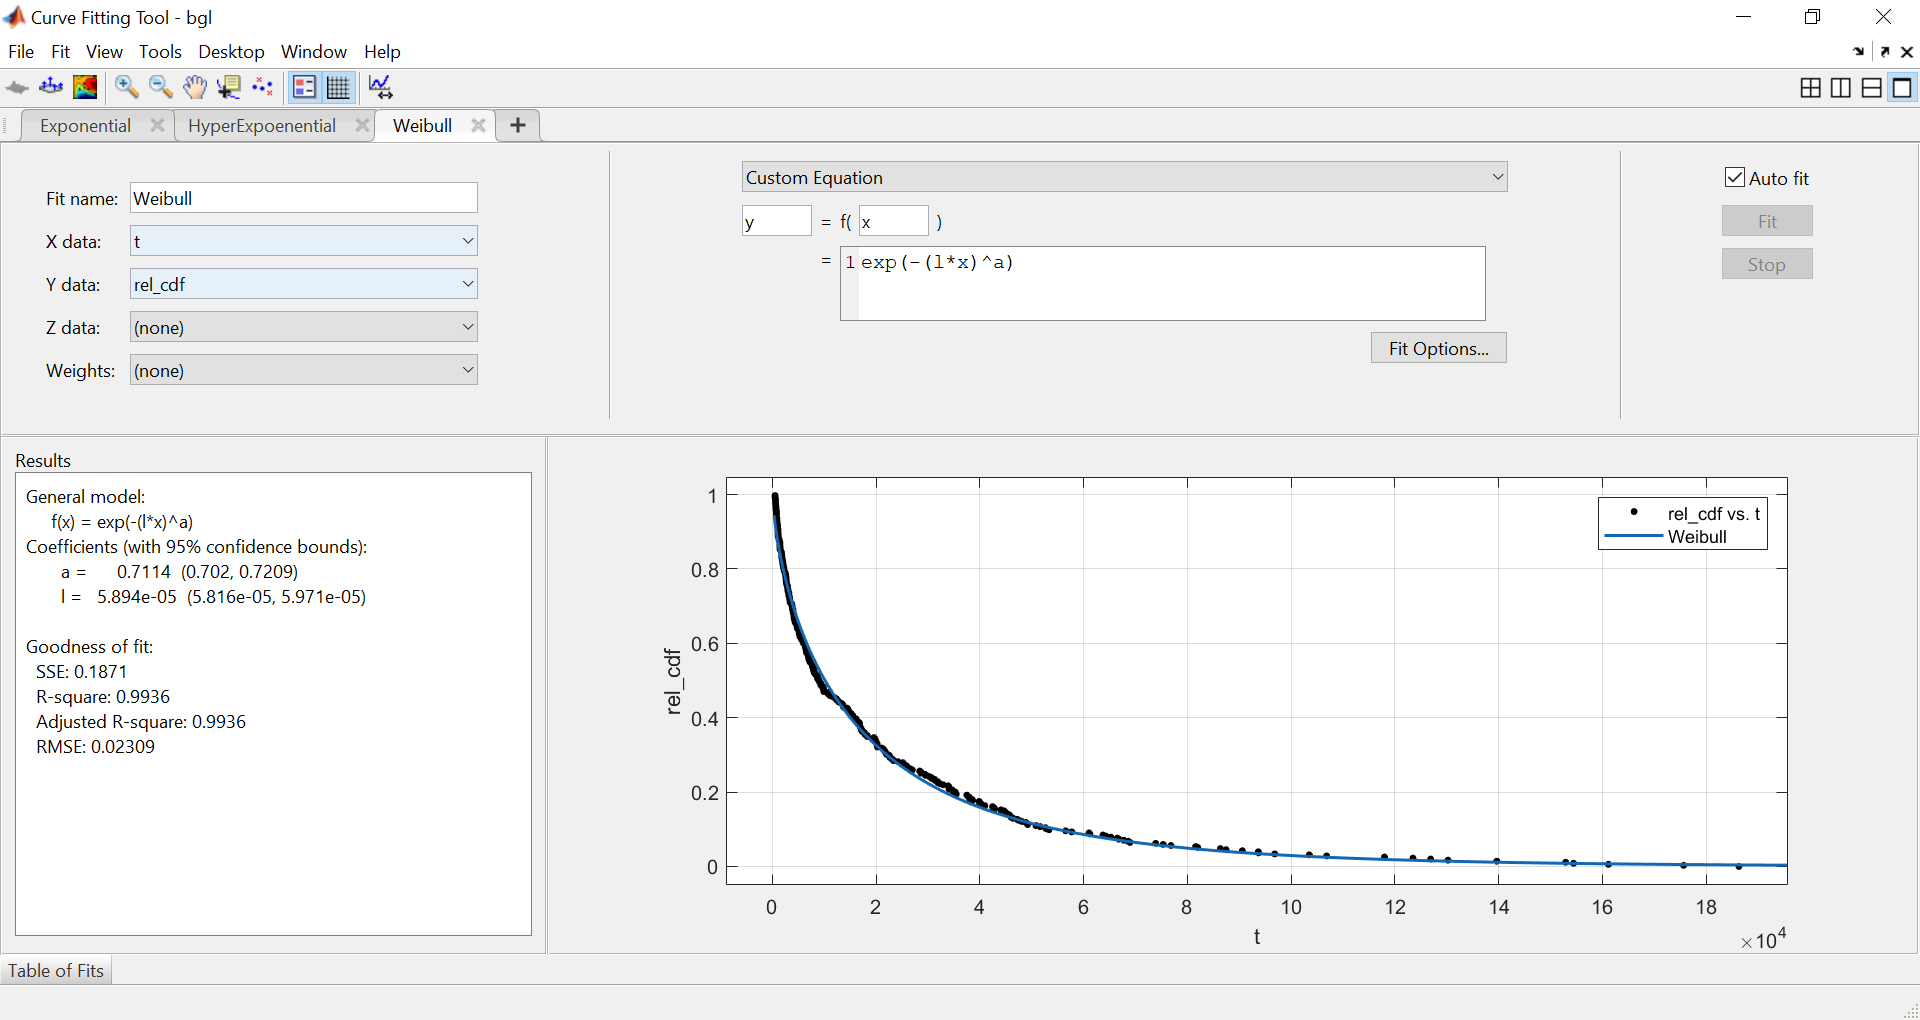
\includegraphics[width=0.9\linewidth,keepaspectratio]{Weibull_bgl}
    \caption{Curve Fitting modello Weibull}
    \label{Weibull_bgl}
  \end{figure}

  Per valutare la bontà del fitting è stato utilizzato il \textbf{Kolmogorov-Smirnov Test}.\\

  \begin{figure}[!htbp]
    \centering
    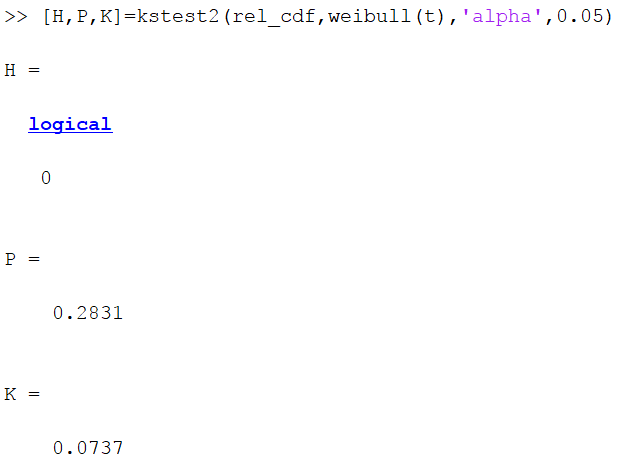
\includegraphics[width=0.4\linewidth,keepaspectratio]{ks_weibull_bgl}
    \caption{Kolmogorov-Smirnov Test Weibull}
    \label{ks_weibull_bgl}
  \end{figure}

  L'ipotesi nulla è valida al 28,31\%, con confidenza del 95\%.\\
  Quindi osservando il valore di R-quadro, è possibile concludere che il
  modello ipotizzato fitta bene la CDF empirica.\\

  \clearpage

  \item \textbf{Iperesponenziale}:
  $$ y = a e^{- \lambda_1  x} +  b  e^{- \lambda_2  x} $$
  Il modello risultante in matlab è riportato nella figura \ref{HyperExponential_bgl}.\\

  \begin{figure}[!htbp]
    \centering
    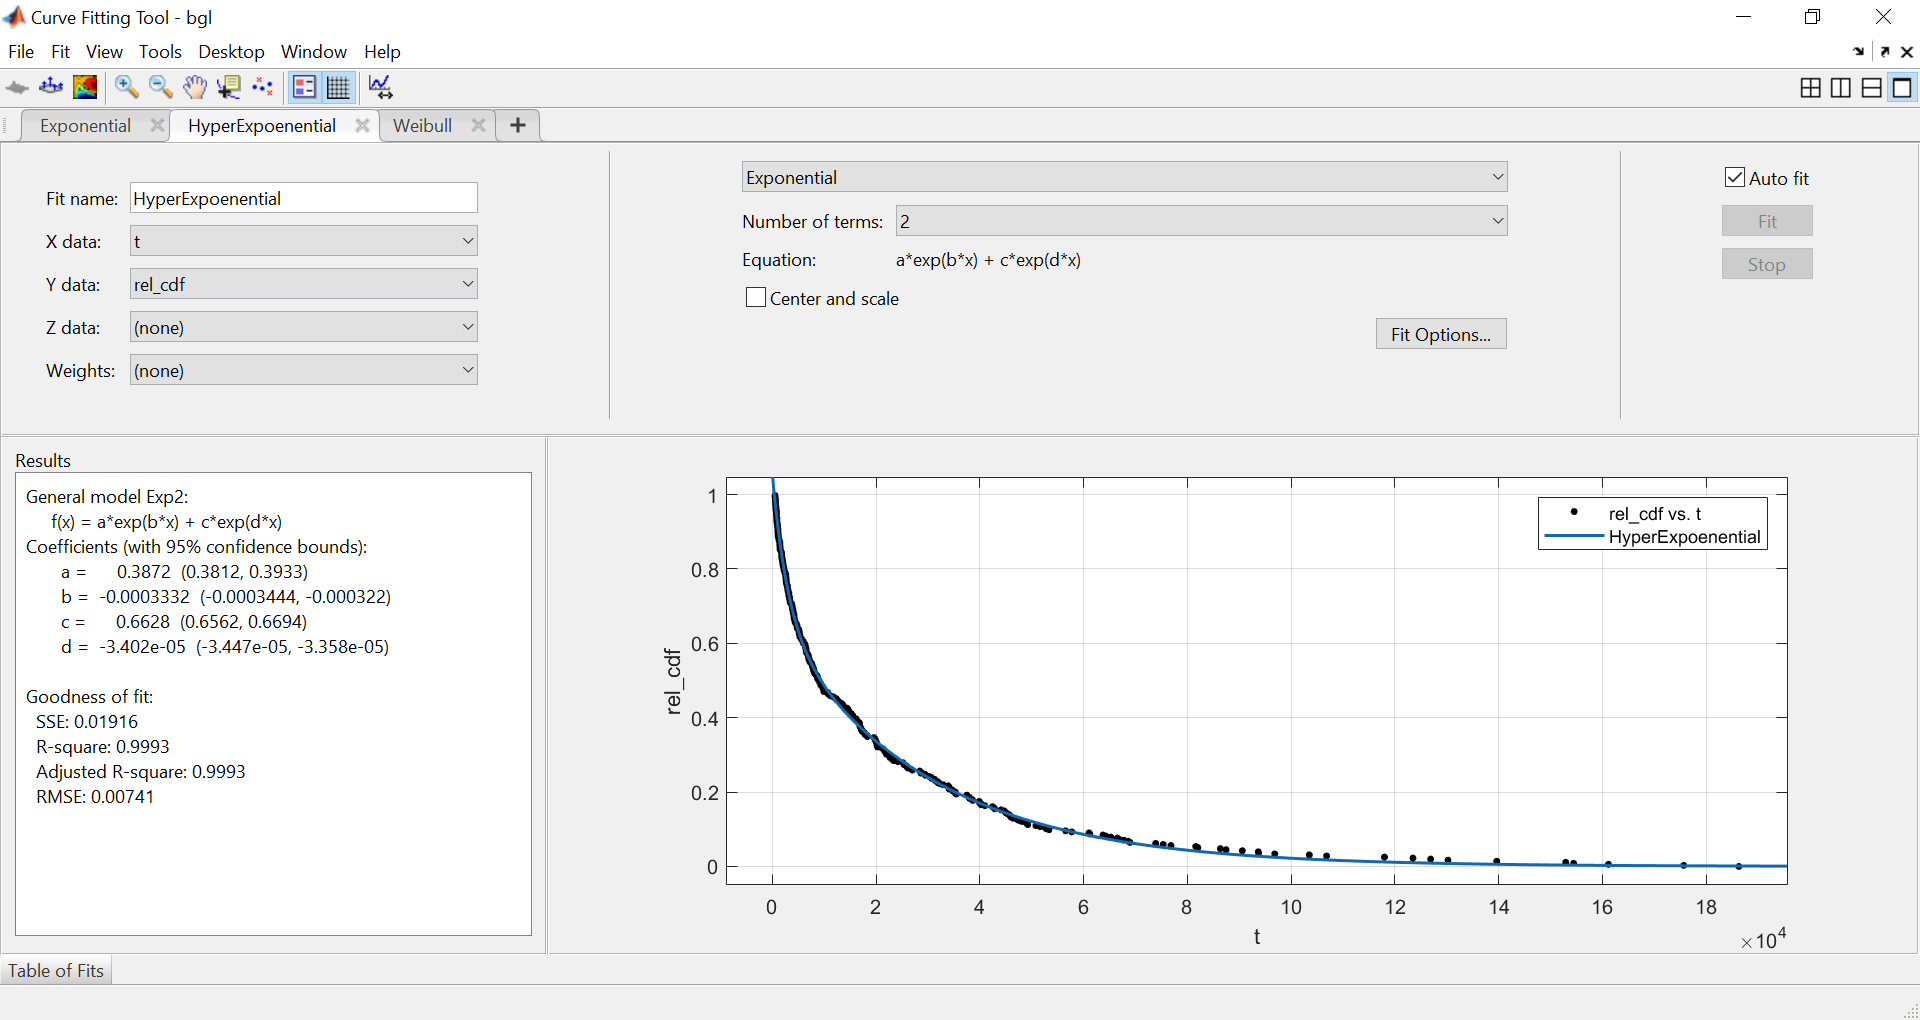
\includegraphics[width=0.9\linewidth,keepaspectratio]{HyperExponential_bgl}
    \caption{Curve Fitting modello iperesponenziale}
    \label{HyperExponential_bgl}
  \end{figure}

  Per valutare la bontà del fitting è stato utilizzato il \textbf{Kolmogorov-Smirnov Test}.\\

  \begin{figure}[!htbp]
    \centering
    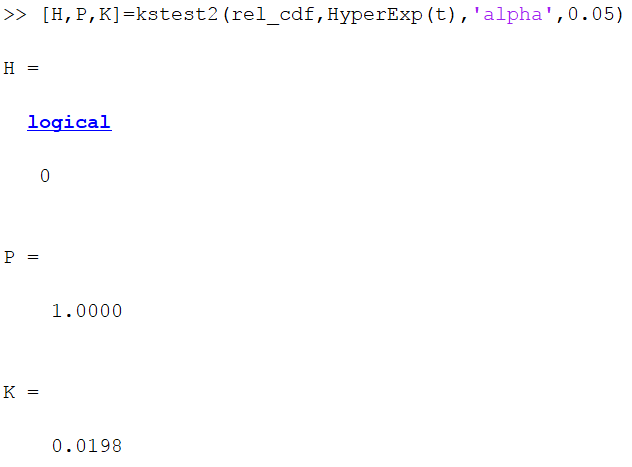
\includegraphics[width=0.5\linewidth,keepaspectratio]{ks_hyperexp_bgl}
    \caption{Kolmogorov-Smirnov Test Weibull}
    \label{ks_hyperexp_bgl}
  \end{figure}

  L'ipotesi è valida al 100\%, con confidenza del 95\%.\\
  Osservando anche il valore di R-quadro (99,93\%), è possibile affermare che
  l'iperesponenziale è il modello migliore per il fitting dei dati a disposizione.\\

  \clearpage
\end{itemize}

\clearpage

\subsection{Analisi del Log}
Nella figura \ref{statistics_bgl} è riportata l'esecuzione dello script
\textit{logStatistics.sh}, che fornisce informazioni sul numero di fallimenti
per categoria e per nodo.\\
Da quest'analisi risulta esserci un collo di bottiglia per le categorie:
\textit{J18-U11 (50055 fallimenti)} ed uno per i nodi: \textit{R71-M0-N4 (1716 fallimenti)}.\\

\begin{figure}[!htbp]
  \centering
  \includegraphics[width=.8\linewidth,keepaspectratio]{statistics_bgl}
  \caption{Esecuzione script logStatistics.txt}
  \label{statistics_bgl}
\end{figure}

\clearpage

\subsection{Domanda 1}
\textit{La finestra di coalescenza CWIN è la stessa per tutti i nodi considerati?}

\subsubsection*{Soluzione}
Per poter rispondere alla domanda è necessario calcolare la finestra di coalescenza
per ogni log filtrato per nodo.
I risultati ottenuti sono riportati in figura \ref{cwin_5_nodi_bgl}.\\

\begin{minipage}{\linewidth}
  \centering
  \begin{minipage}{0.49\linewidth}
    \begin{figure}[H]
      \includegraphics[width=\linewidth]{plot_CWIN_R71-M0-N4}
      \caption*{r71}
    \end{figure}
  \end{minipage}
  \begin{minipage}{0.49\linewidth}
    \begin{figure}[H]
      \includegraphics[width=\linewidth]{plot_CWIN_R12-M0-N0}
      \caption*{r12}
    \end{figure}
  \end{minipage}
  \begin{minipage}{0.49\linewidth}
    \begin{figure}[H]
      \includegraphics[width=\linewidth]{plot_CWIN_R63_M0-N2}
      \caption*{r63-n2}
    \end{figure}
  \end{minipage}
  \begin{minipage}{0.49\linewidth}
    \begin{figure}[H]
      \centering
      \includegraphics[width=.8\linewidth]{plot_CWIN_R03_M1_NF}
      \caption*{r03}
    \end{figure}
  \end{minipage}
  \begin{minipage}{0.49\linewidth}
    \hspace{0.25\linewidth}
    \begin{figure}[H]
      \includegraphics[width=\linewidth]{plot_CWIN_R63_M0-N0}
      \caption*{r63-n0}
    \end{figure}
  \end{minipage}
\end{minipage}
\captionof{figure}{CWIN: log filtrato per Nodo}
\label{cwin_5_nodi_bgl}

\clearpage

Dalla seguente tabella si osserva che non è possibile scegliere un
valore univoco di finestra di coalescenza per tutti i nodi considerati, in quanto
i valori differiscono eccessivamente tra di loro.\\
Imponendo un unico valore di CWIN si potrebbe incorrere in problematiche di
collisioni tra differenti eventi di fallimento.\\

\begin{figure}[!htbp]
  \centering
  \includegraphics[width=.5\linewidth,keepaspectratio]{node_cwin_bgl}
  \caption{Tabella fallimenti per categorie e nodi}
  \label{node_cwin_bgl}
\end{figure}

\clearpage

In seguito è riportato il confronto tra la reliability del sistema e quella dei
nodi che, fissato il valore CWIN, presentano più di 30 tuple.\\

\begin{minipage}{\linewidth}
  \centering
  \begin{minipage}{.49\linewidth}
    \begin{figure}[H]
      \includegraphics[width=\linewidth]{interarrivals_R71-M0-N4}
      \caption*{R71}
    \end{figure}
  \end{minipage}
  \begin{minipage}{.49\linewidth}
    \begin{figure}[H]
      \includegraphics[width=\linewidth]{interarrivals_R12-M0-N0}
      \caption*{R12}
    \end{figure}
  \end{minipage}
  \begin{minipage}{.49\linewidth}
    \hspace{0.25\linewidth}
    \begin{figure}[H]
      \includegraphics[width=\linewidth]{interarrivals_R63-M0-N0}
      \caption*{R63}
    \end{figure}
  \end{minipage}
\end{minipage}
\captionof{figure}{Confronto Reliability Sistema e Nodi}

\clearpage

\subsection{Domanda 2}
\textit{Analizzare le categorie J18-U01 e J18-U11, calcolando il tuple count e
i modelli di reliability}

\textit{Tuple Count}:

\begin{minipage}{\linewidth}
  \begin{minipage}{\linewidth}
    \begin{figure}[H]
      \includegraphics[width=\linewidth]{plot_CWIN_J18_U01}
      \caption*{J18-U01}
    \end{figure}
  \end{minipage}
  \begin{minipage}{\linewidth}
    \begin{figure}[H]
      \includegraphics[width=\linewidth]{plot_CWIN_J18_U11}
      \caption*{J18-U11}
    \end{figure}
  \end{minipage}
\end{minipage}
\captionof{figure}{CWIN: log filtrato per categoria errore}

\clearpage

\textit{Modelli di Reliability}:

\begin{minipage}{\linewidth}
  \centering
  \begin{minipage}{.7\linewidth}
    \begin{figure}[H]
      \includegraphics[width=\linewidth]{rel_U01}
      \caption*{J18-U01}
    \end{figure}
  \end{minipage}

  \begin{minipage}{.7\linewidth}
    \begin{figure}[H]
      \includegraphics[width=\linewidth]{rel_U11}
      \caption*{J18-U11}
    \end{figure}
  \end{minipage}
\end{minipage}
\captionof{figure}{Modelli di Reliability}

\clearpage

\subsection{Domanda 3}
\textit{What are the most entries-prone racks/nodes?}\\

\subsubsection*{Soluzione}

 Per ottenere la lista dei nodi, delle categorie e dei rack è stato utilizzato lo Script
 \textit{logStatistics.sh}, con l'aggiunta del seguente codice per visualizzare
 i rack.\\

\begin{lstlisting}[language=bash]
echo "== Breakup by RACK =="
cat $1 | awk '{print substr($2,1,3)}' | sort | uniq -c | sort -nr | head -n 5 | awk '{print $2, $1}'
echo " * only the 5 most occurring racks are reported"
echo ""
\end{lstlisting}

L'output ottenuto è riportato in figura \ref{u6}.\\

\begin{figure}[!htbp]
  \centering
  \includegraphics[width=\linewidth,keepaspectratio]{u6}
  \caption{Report Script logStatistics.sh}
  \label{u6}
\end{figure}
